% ******************************* PhD Thesis Template **************************
% Spellchecker ignore
% cSpell:ignore draftclassic, custommargin, customfont, authoryear, custombib, natbib, biblatex, Uncomment, ifdefine, includeonly, Frontmatter, frontmatter, listoffigures, listoftables, printnomenclature, mainmatter, Backmatter, backmatter, plainnat, cleardoublepage, uncomment, printbibliography, bibintoc, printthesisindex (1)
% Please have a look at the README.md file for info on how to use the template
\documentclass[a4paper,11pt,numbered,print,index]{Classes/PhDThesisPSnPDF}

% ******************************************************************************
% ******************************* Class Options ********************************
% *********************** See README for more details **************************
% ******************************************************************************

% `a4paper'(The University of Cambridge PhD thesis guidelines recommends a page
% size a4 - default option) or `a5paper': A5 Paper size is also allowed as per
% the Cambridge University Engineering Department guidelines for PhD thesis
%
% `11pt' or `12pt'(default): Font Size 10pt is NOT recommended by the University
% guidelines
%
% `oneside' or `twoside'(default): Printing double side (twoside) or single
% side.
%
% `print': Use `print' for print version with appropriate margins and page
% layout. Leaving the options field blank will activate Online version.
%
% `index': For index at the end of the thesis
%
% `draftclassic': For draft mode without loading any images (same as draft in book)
%
% `draft': Special draft mode with line numbers, images, and water mark with
% timestamp and custom text. Position of the text can also be modified.
%
% `abstract': To generate only the title page and abstract page with
% dissertation title and name, to submit to the Student Registry
%
% `chapter`: This option enables only the specified chapter and it's references
%  Useful for review and corrections.
%
% ************************* Custom Page Margins ********************************
%
% `custommargin`: Use `custommargin' in options to activate custom page margins,
% which can be defined in the preamble.tex. Custom margin will override
% print/online margin setup.
%
% *********************** Choosing the Fonts in Class Options ******************
%
% `times' : Times font with math support. (The Cambridge University guidelines
% recommend using times)
%
% `fourier': Utopia Font with Fourier Math font (Font has to be installed)
%            It's a free font.
%
% `customfont': Use `customfont' option in the document class and load the
% package in the preamble.tex
%
% default or leave empty: `Latin Modern' font will be loaded.
%
% ********************** Choosing the Bibliography style ***********************
%
% `authoryear': For author-year citation eg., Krishna (2013)
%
% `numbered': (Default Option) For numbered and sorted citation e.g., [1,5,2]
%
% `custombib': Define your own bibliography style in the `preamble.tex' file.
%              `\RequirePackage[square, sort, numbers, authoryear]{natbib}'.
%              This can be also used to load biblatex instead of natbib
%              (See Preamble)
%
% **************************** Choosing the Page Style *************************
%
% `default (leave empty)': For Page Numbers in Header (Left Even, Right Odd) and
% Chapter Name in Header (Right Even) and Section Name (Left Odd). Blank Footer.
%
% `PageStyleI': Chapter Name next & Page Number on Even Side (Left Even).
% Section Name & Page Number in Header on Odd Side (Right Odd). Footer is empty.
%
% `PageStyleII': Chapter Name on Even Side (Left Even) in Header. Section Number
% and Section Name in Header on Odd Side (Right Odd). Page numbering in footer

% Uncomment to change page style
%\pagestyle{PageStyleII}

% ********************************** Preamble **********************************
% Preamble: Contains packages and user-defined commands and settings
% Spellchecker ignore
% cSpell:ignore cmmnt, ignorespaces, belowdisplayskip, abovedisplayskip, bigints, custommargin, innerside, outerside, topmargin, ifset, parskip, whitespaces, raggedbottom, enumitem, setlist, topsep, customfont, helvet, setmainfont, opentype, Semibold, newfontfamily, libertinesystemfont, Pseudocode, algpseudocode, Hyperreferencing, labelsep, tableposition, figurename, labelfont, captionsetup, wrapfig, Uncomment, restylefloat, Subcaption, uncommenting, texlive, subcaption, booktabs, multirow, multicol, longtable, tabularx, siunitx, linespacing, doublespacing, onehalfspacing, singlespacing, clubpenalty, widowpenalty, perpage, footmisc, xfrac, mathl, cmsy, Lorentzian, cleveref, custombib, authoryear, natbib, biblatex, natbibpackage, backend, biber, citestyle, bibname, contentsname, listfigurename, listtablename, setcounter, secnumdepth, tocdepth, uncomment, nomname, appendixtocname, appendixpagename, appendixname, Appndx, setkeys, grayscale, todonotes, colorinlistoftodos, mynote, listoftodos, mathrm
% ******************************************************************************
% ****************************** Custom Margin *********************************

% Add `custommargin' in the document class options to use this section
% Set {innerside margin / outerside margin / topmargin / bottom margin}  and
% other page dimensions
\ifsetCustomMargin{}
  \RequirePackage[left=37mm,right=30mm,top=35mm,bottom=30mm]{geometry}
  \setFancyHdr{} % To apply fancy header after geometry package is loaded
\fi

% Add spaces between paragraphs
%\setlength{\parskip}{0.5em}
% Ragged bottom avoids extra whitespaces between paragraphs
\raggedbottom{}
% To remove the excess top spacing for enumeration, list and description
%\usepackage{enumitem}
%\setlist[enumerate,itemize,description]{topsep=0em}

% *****************************************************************************
% ******************* Fonts (like different typewriter fonts etc.)*************

% Add `customfont' in the document class option to use this section

\ifsetCustomFont{}
  % Set your custom font here and use `customfont' in options. Leave empty to
  % load computer modern font (default LaTeX font).
  %\RequirePackage{helvet}

  % For use with XeLaTeX
  %  \setmainfont[
  %    Path              = ./libertine/opentype/,
  %    Extension         = .otf,
  %    UprightFont = LinLibertine_R,
  %    BoldFont = LinLibertine_RZ, % Linux Libertine O Regular Semibold
  %    ItalicFont = LinLibertine_RI,
  %    BoldItalicFont = LinLibertine_RZI, % Linux Libertine O Regular Semibold Italic
  %  ]
  %  {libertine}
  %  % load font from system font
  %  \newfontfamily\libertinesystemfont{Linux Libertine O}
\fi

% *****************************************************************************
% **************************** Custom Packages ********************************

% ************************* Algorithms and Pseudocode **************************

%\usepackage{algpseudocode}


% ********************Captions and Hyperreferencing / URL **********************

% Captions: This makes captions of figures use a boldfaced small font.
%\RequirePackage[small,bf]{caption}

\RequirePackage[labelsep=space,tableposition=top]{caption}
\renewcommand{\figurename}{Fig.} %to support older versions of captions.sty
\usepackage[font=small,labelfont=bf]{caption}

% This package lets you refer to a chapter
\usepackage{hyperref}

%\usepackage{caption}
%\captionsetup[table]{position=bottom} % Caption below table

% *************************** Graphics and figures *****************************

%\usepackage{rotating}
\usepackage{wrapfig}

% Uncomment the following two lines to force Latex to place the figure.
% Use [H] when including graphics. Note 'H' instead of 'h'
\usepackage{float}
%\restylefloat{figure}

% Subcaption package is also available in the sty folder you can use that by
% uncommenting the following line
% This is for people stuck with older versions of texlive
%\usepackage{sty/caption/subcaption}
\usepackage{subcaption}

% ********************************** Tables ************************************
\usepackage{booktabs} % For professional looking tables
\usepackage{multirow}

%\usepackage{multicol}
%\usepackage{longtable}
%\usepackage{tabularx}


% *********************************** SI Units *********************************
\usepackage{siunitx} % use this package module for SI units


% ******************************* Line Spacing *********************************

% Choose linespacing as appropriate. Default is one-half line spacing as per the
% University guidelines

% \doublespacing
% \onehalfspacing
% \singlespacing


% ************************ Formatting / Footnote *******************************

% Don't break enumeration (etc.) across pages in an ugly manner (default 10000)
%\clubpenalty=500
%\widowpenalty=500

%\usepackage[perpage]{footmisc} %Range of footnote options

\newcommand{\cmmnt}[1]{\ignorespaces} % command function

\setlength{\abovedisplayskip}{10pt} % For spacing above align segment
\setlength{\belowdisplayskip}{10pt} % For spacing below align segment 

\setlength{\parindent}{2ex} % Paragraph indent on first row

% Math packages and commands
\usepackage{bigints}
\usepackage{xfrac}
\newcommand{\ket}[1]{\(\left|#1\right\rangle \)}
\newcommand{\dd}{\mathrm{d}}


\DeclareMathAlphabet\mathl{OMS}{cmsy}{b}{n} % for Lorentzian L(v,v')


% *****************************************************************************
% *************************** Bibliography  and References ********************

%\usepackage{cleveref} %Referencing without need to explicitly state fig /table

% Add `custombib' in the document class option to use this section
\ifuseCustomBib{}
   \RequirePackage[square, sort, numbers, authoryear]{natbib} % CustomBib

% If you would like to use biblatex for your reference management, as opposed 
% to the default `natbibpackage` pass the option `custombib` in the document class. 
% Comment out the previous line to make sure you don't load the natbib package. 
% Uncomment the following lines and specify the location of references.bib file

%\RequirePackage[backend=biber, style=numeric-comp, citestyle=numeric, sorting=nty, natbib=true]{biblatex}
%\bibliography{References/references} %Location of references.bib only for biblatex

\fi

% changes the default name `Bibliography` -> `References'
\renewcommand{\bibname}{References}


% ******************************************************************************
% ************************* User Defined Commands ******************************
% ******************************************************************************

% *********** To change the name of Table of Contents / LOF and LOT ************

%\renewcommand{\contentsname}{My Table of Contents}
%\renewcommand{\listfigurename}{My List of Figures}
%\renewcommand{\listtablename}{My List of Tables}


% ********************** TOC depth and numbering depth *************************

\setcounter{secnumdepth}{2}
\setcounter{tocdepth}{2}


% ******************************* Nomenclature *********************************

% To change the name of the Nomenclature section, uncomment the following line

%\renewcommand{\nomname}{Symbols}


% ********************************* Appendix ***********************************

% The default value of both \appendixtocname and \appendixpagename is `Appendices'. These names can all be changed via:

%\renewcommand{\appendixtocname}{List of appendices}
%\renewcommand{\appendixname}{Appndx}

% *********************** Configure Draft Mode **********************************

% Uncomment to disable figures in `draft'
%\setkeys{Gin}{draft=true}  % set draft to false to enable figures in `draft'

% These options are active only during the draft mode
% Default text is "Draft"
%\SetDraftText{DRAFT}

% Default Watermark location is top. Location (top/bottom)
%\SetDraftWMPosition{bottom}

% Draft Version - default is v1.0
%\SetDraftVersion{v1.1}

% Draft Text grayscale value (should be between 0-black and 1-white)
% Default value is 0.75
%\SetDraftGrayScale{0.8}


% ******************************** Todo Notes **********************************
%% Uncomment the following lines to have todonotes.

%\ifsetDraft
%	\usepackage[colorinlistoftodos]{todonotes}
%	\newcommand{\mynote}[1]{\todo[author=kks32,size=\small,inline,color=green!40]{#1}}
%\else
%	\newcommand{\mynote}[1]{}
%	\newcommand{\listoftodos}{}
%\fi

% Example todo: \mynote{Hey! I have a note}


% ************************ Thesis Information & Meta-data **********************
% Thesis title and author information, reference file for biblatex
% ************************ Thesis Information & Meta-data **********************
%% The title of the thesis
\title{I dont know yet}
%\texorpdfstring is used for PDF metadata. Usage:
%\texorpdfstring{LaTeX_Version}{PDF Version (non-latex)} eg.,
%\texorpdfstring{$sigma$}{sigma}

%% Subtitle (Optional)
%\subtitle{Using the CUED template}

%% The full name of the author
\author{Faustmann Christian}

%% Department (eg. Department of Engineering, Maths, Physics)
\dept{Faculty of Physics}

%% University and Crest
\university{Technical University of Vienna}
% Crest minimum should be 30mm.
\crest{
\includegraphics[width=0.2\textwidth]{TU_Signet}}
%% Use this crest, if you are using the college crest
%% Crest long miminum should be 65mm
%\crest{\includegraphics[width=0.45\textwidth]{University_Crest_Long}}

%% College shield [optional] 
% Crest minimum should be 30mm.
%\collegeshield{\includegraphics[width=0.2\textwidth]{CollegeShields/Kings}}


%% Supervisor (optional)
%% for multiple supervisors, append each supervisor with the \newline command
%\supervisor{Prof. A.B. Supervisor\newline
%Prof. C.D. Supervisor}

%% Supervisor Role (optional) - Supervisor (default) or advisor
% \supervisorrole{\textbf{Supervisors: }}
%% if no title is desired:
% \supervisorrole{}

%% Supervisor line width: required to align supervisors
%\supervisorlinewidth{0.35\textwidth}

%% Advisor (optional)
%% for multiple advisors, append each advisor with the \newline command
%\advisor{Dr. A. Advisor\newline
%Dr. B. Advisor}
     
%% Advisor Role (optional) - Advisor (default) or leave empty
% \advisorrole{Advisors: }
%% if no title is required
% \advisorrole{}

%% Advisor line width: required to align supervisors
%\advisorlinewidth{0.25\textwidth}


%% You can redefine the submission text:
% Default as per the University guidelines:
% ``This dissertation is submitted for the degree of''
%\renewcommand{\submissiontext}{change the default text here if needed}

%% Full title of the Degree
\degreetitle{Bachelor of Science}

%% College affiliation (optional)
\college{TU Vienna}

%% Submission date
% Default is set as {\monthname[\the\month]\space\the\year}
%\degreedate{September 2014} 

%% Meta information
\subject{LaTeX} \keywords{{LaTeX} {PhD Thesis} {Engineering} {University of
Cambridge}}


% ***************************** Abstract Separate ******************************
% To printout only the titlepage and the abstract with the PhD title and the
% author name for submission to the Student Registry, use the `abstract' option in
% the document class.

\ifdefineAbstract{}
 \pagestyle{empty}
 \includeonly{Declaration/declaration, Abstract/abstract}
\fi

% ***************************** Chapter Mode ***********************************
% The chapter mode allows user to only print particular chapters with references
% Title, Contents, Frontmatter are disabled by default
% Useful option to review a particular chapter or to send it to supervisor.
% To use choose `chapter' option in the document class

\ifdefineChapter{}
 \includeonly{Chapter3/chapter3}
\fi

% ******************************** Front Matter ********************************
\begin{document}

\frontmatter

\maketitle

%\include{Dedication/dedication}
%\include{Declaration/declaration}
%\include{Acknowledgement/acknowledgement}
%% ************************** Thesis Abstract *****************************
% Use `abstract' as an option in the document class to print only the titlepage and the abstract.
\begin{abstract}
This is where you write your abstract ...
\end{abstract}

%!TEX root = ../thesis.tex
% Spellchecker ignore
% cSpell:ignore Lett, detuned, nano, retroreflection, includegraphics, ifpdf, graphicspath, Rauschenbeutel, nanowaveguides, microresonator, signicant, nanofiber, textasciitilde, autoref
%*******************************************************************************
%****************************** Introduction ***********************************
%*******************************************************************************

\chapter*{Introduction}

% **************************** Define Graphics Path **************************
\ifpdf{}
    \graphicspath{{Introduction/Figs/Raster/}{Introduction/Figs/PDF/}{Introduction/Figs/}}
\else
    \graphicspath{{Introduction/Figs/Vector/}{Introduction/Figs/}}
\fi

\begin{figure}[hb]
    \centering
    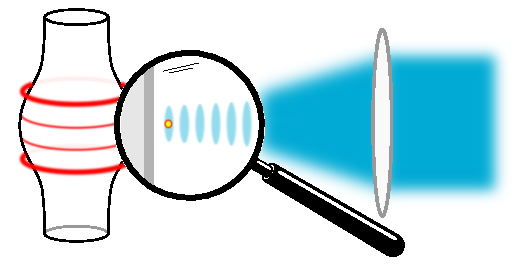
\includegraphics[width=0.6\textwidth]{resonator_trap}
    \caption{\label{fig:resonator_trap} Schematic representation of a WGM 
    resonator and a optical dipole trap}
\end{figure}
One of Prof.\ Rauschenbeutel projects uses a novel type of whispering-gallery-mode (WGM)
resonator interfaced via nanowaveguides and coupled to single Rubidium atoms to 
carry out experiments in the realm of Cavity Quantum Electrodynamics. The WGM 
resonator is a so-called bottle-microresonator (BMR) manufactured from a standard 
optical glass fiber in a heat and pull process. The light is radially confined 
inside the resonator by total internal reflection and propagates along the 
circumference of the resonator. In such a structure, a signicant fraction of the 
light field propagates in the evanescent field. By overlapping this field with 
the evanescent field of an optical nanofiber, light can be coupled into and out 
of the resonator very efficiently. Due to the extremely low absorption of silica 
(and low surface roughness) we can produce bottle-resonators with ultra-high 
optical Q-factor exceeding 10\(^{8}\). Rubidium atoms are delivered to the 
resonator using an atomic fountain. When the atoms enter the vicinity of the WGM, 
and they are in the evanescent field they can be strongly coupled to the light. 
For the moment the \(^{85}Rb\) atoms are only flying by the resonator for 
\textasciitilde{}\SI{2}{\micro\second}. Moreover the distance between the 
resonator and the atom is not controlled. This uncertainty induces fluctuations
on the atom-resonator coupling from shot to shot and limits the efficiency of the
different devices demonstrated with the setup. The short duration of the atom
light interaction also prevents the manipulation of the atomic state, necessary
for the realization of complex quantum information protocols such as two photon
gates~\cite{PhysRevLett.92.127902}. The solution would be to trap the atom at the
vicinity of the BMR\@. The choice made to trap the atom is to use a dipole trap 
created from the retroreflection of a focused beam on the resonator surface 
inspired from~\cite{Thompson1202} (see Fig.~\ref{fig:resonator_trap}). Due to the 
experiment configuration, the trap can not be loaded from a dense cloud, but only 
from the atoms flying next to the resonator, which have a non-zero velocity, which 
further implies that a big trap depth is needed. The usual dipole traps are built 
with lasers detuned from the transition between the ground and the first excited 
state. But this would create a trap too far from the resonator and thus in this 
thesis, we discuss the possibility to realise a trap detuned from the second exited 
state of \(^{85}\)Rb which has transitions at \(\lambda \approx \SI{420}{\nano\meter} \).
In this thesis, we will also evaluate the parameters needed for such a trap, and 
then report on an absorption spectroscopy measurement leading to the estimation 
of the saturation intensity of the \(5S_{1/2}\) to \(6P_{3/2}\) transition.

% *********************** Adding TOC and List of Figures ***********************

\tableofcontents

\listoffigures

\listoftables

% \printnomenclature[space] space can be set as 2em between symbol and description
%\printnomenclature[3em]

\printnomenclature{}

% ******************************** Main Matter *********************************
\mainmatter{}

%!TEX root = ../thesis.tex
% Spellchecker ignore
% cSpell:ignore ifpdf, graphicspath, detuned, bigskip, nano, citep, milli, detuning, medskip, mathrm
%*******************************************************************************
%****************************** First Chapter **********************************
%*******************************************************************************

\chapter{\label{chap:dipole}Theory of laser trapping of atoms}


\ifpdf{}
    \graphicspath{{Chapter1/Figs/Raster/}{Chapter1/Figs/PDF/}{Chapter1/Figs/}}
\else
    \graphicspath{{Chapter1/Figs/Vector/}{Chapter1/Figs/}}
\fi

The strategy pursued to trap is a optical dipole trap. For that the laser light 
needs to be detuned from a resonance of the atom. Thereafter the atoms are trapped
to the maxima of intensity for a red detuned laser. The beam will be reflected 
from the resonator surface and creates thereby a standing wave. The 1\(^{st}\)
maxima is at \(\sfrac{1}{4}~\lambda_{trap} \).
\bigskip

So how to choose \(\lambda_{trap}\)?
\bigskip

Because of the interaction with the BMR evanescent field the atoms need to
be trapped really close: \(\lambda / 2\pi \approx \SI{130}{\nano\meter} \) \\
Most common resonance of rubidium is \(5S_{1/2} \rightarrow 5P_{3/2}\) @
\SI{780.24}{\nano\meter}. If we use a laser red-detuned from \(\lambda \) = 
\SI{780.24}{\nano\meter} then our first maxima would be at \SI{195}{\nano\meter}
\(\Rightarrow \) Not close enough!
\bigskip

But rubidium has another transition from \(5S_{1/2} \rightarrow 6P_{3/2}\) @
\SI{420.29}{\nano\meter}, which leads to a distance of \SI{105}{\nano\meter} from
the BMR to the 1\(^{st}\) maxima. But in the formula \citep{grimm} of the trap potential (\(U_{dip}\))
arises the transition strength (\(\Gamma_\omega \)) of this specific transition:
\bigskip
\begin{align}
    U_\mathrm{dip}(\mathrm{z})=-\frac{\pi c^2}{2\omega_0^3} \left( \frac{2\Gamma_{\omega,\mathrm{D2}}}{\Delta_{\mathrm{D2}}} + \frac{\Gamma_{\omega,\mathrm{D1}}}{\Delta_{\mathrm{D1}}}\right) I(\mathrm{z})
\end{align}
\bigskip
We have to compare this potential to the kinetic energy of our rubidium atoms. The atoms fall approximately
\SI{60}{\milli\second} and the corresponding kinetic energy would be \(E_{kin} = \frac{1}{2} m_{Rb} v^2\).
In terms of temperature we would get: \(E_{kin} / k_B = \SI{1.77}{\milli\kelvin} \). This is quite huge
for a dipole trap. For that reason one needs to know \(\Gamma_{\omega,420nm-Line} \) and one also needs to have a trap
with a small detuning. This requires to see the transitions to have a reference to lock the laser afterwards.
\bigskip
To determine \(\Gamma_{\omega,420nm-Line} \) we can use a theoretical relation with the intensity saturation, which has to be checked by our measurement:
\begin{align}
    I_{s,420} &= \frac{\Gamma_{\omega,tot,420}\cdot{\omega_{420}}^3\cdot I_{s,780}}{\Gamma_{\omega,420}\cdot\Gamma_{\omega,780}\cdot{\omega_{780}}^3}
\end{align}
\begin{align*}
    \text{with~~~} \Gamma_{\omega,tot,420} &= \frac{1}{total~lifetime~of~6P_{3/2}~state}
\end{align*}
\medskip


\(\Rightarrow \) We want to measure \(I_{s}\) for the blue \SI{420.29}{\nano\meter}-line. 


%!TEX root = ../thesis.tex
% Spellcheck ignore
% cSpell:ignore realrubidium, giga, levelscheme, deexcite, eqref, weakfield, intlorgau, gauvslor, atomicmassunit, citep, ifpdf, graphicspath, bigskip, minipage, includegraphics, twolevel, captionof, nano, FWHM, linewidth, electronvolt, Linewidth, nlinewidth, Lorentzian, pagebreak, wrapfigure, photodiode, mathrm, itemsep, extracolsep, toprule, multicolumn, midrule, bottomrule, energylevel, hyperfine, groundstate, nist, groundstates, nonumber, Lorentzians
%*******************************************************************************
%****************************** Second Chapter *********************************
%*******************************************************************************

\ifpdf{}
\graphicspath{{Chapter2/Figs/Raster/}{Chapter2/Figs/PDF/}{Chapter2/Figs/}}
\else
\graphicspath{{Chapter2/Figs/Vector/}{Chapter2/Figs/}}
\fi

\chapter{Absorption of photon by an atom}  %Title of the Second Chapter
The purpose of this section is to outline the basic features observed in 
saturated absorption spectroscopy and relate them to simple atomic and laser 
physics principles. For this we will follow the guidance of \citep{SAS} and 
\citep{SAS_appendix}.

Electrons can orbit around the atom nucleus following different trajectories which
are quantified, the so called orbitals. It is energetically preferable that the
electron orbit around the atomic nucleus in the lowest possible orbitals, but it 
is possible to excite the electron in different higher excited states. The 
difference of energy states are in the range of typically optical frequencies, 
which give rise to an absorption spectrum. The atomic transitions are sufficiently 
separated such that, when probing close to one resonance, one can consider that 
they behave as a 2 level system.

%********************************** % First Section  *************************************
\section{Laser interactions~-~Two-level atom} %Section - 2.1

We begin with the interaction between a laser field and a sample of stationary 
atoms having only two possible energy levels. Aspects of thermal motion will 
be treated subsequently.\\ 
The ground state is denoted \ket{g} of energy \(E_0 \) and the excited state 
\ket{e} of energy \(E_1 \). The transition frequency \(\nu_0 \) is given by 
Planck's law
\begin{align}
    h \nu_0 = E_1 - E_0~.
\end{align}
For the considered transition, \(\nu_0 \) is in the optical domain.
There can three transition processes happen, as described in Fig.~\ref{fig:twolevel}:
\pagebreak

\begin{figure}[h]
    \centering
    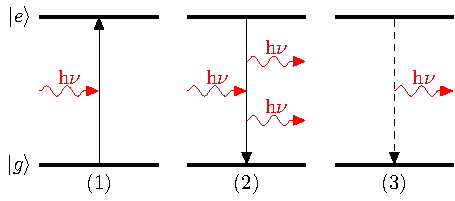
\includegraphics[width=0.6\textwidth]{twolevel}
    \caption{\label{fig:twolevel}Two-level atom model}
\end{figure}


\begin{itemize}
\item[(1)] \textit{absorption}: Atom in the ground state absorbs a photon with 
    the energy \(h \nu_0 \) and is excited. The absorption process is described
    by a transition rate or probability per unit time and is proportional to the
    laser intensity \textit{I} (SI units of \si{\watt\per\meter\squared}) and is
    only significantly different from zero when the laser frequency \(\nu \) is
    near the resonance frequency \(\nu_0 \) of the transition. This transition
    rate will be denoted \(\alpha~I \), where

    \bigskip
    \begin{minipage}[c][][c]{.45\textwidth}
        \begin{align}\label{eq:alpha}
            \alpha = \alpha_0~\mathcal{L}(\nu,\nu_0)
        \end{align}
        and
        \begin{align}
            \mathcal{L}(\nu,\nu_0) &= \frac{1}{ 1+4~{(\nu-\nu_0)}^2 / {\Gamma_\nu}^2 }
        \end{align}
    \end{minipage}
    \hfill
    \begin{minipage}[c]{.45\textwidth}
        \centering
        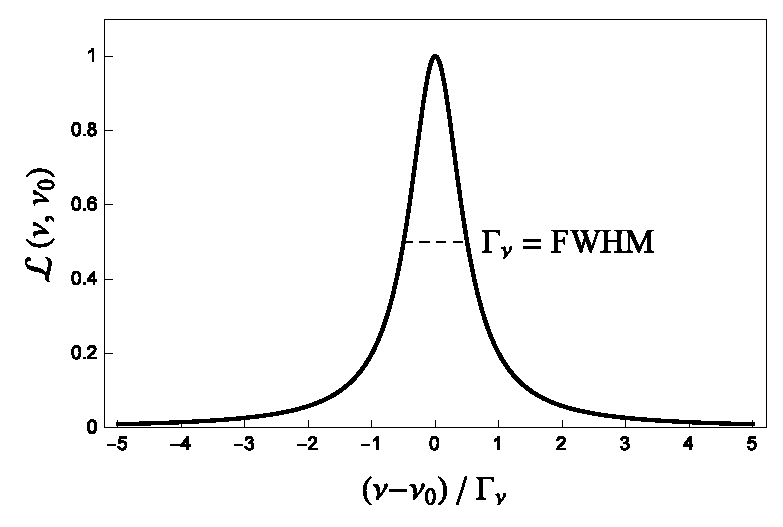
\includegraphics[width=.9\textwidth]{nLinewidth}
        \captionof{figure}{\label{fig:nlinewidth} The Lorentzian line shape profile 
            for a transition}
    \end{minipage}

    \bigskip
    gives the \textit{Lorentzian} frequency dependence with a full width at half
    maximum (FWHM) or \textit{natural linewidth} \(\Gamma_\nu \) of this transition 
    as shown in Fig.~\ref{fig:nlinewidth}. The maximum transition rate \(\alpha_0~I \) 
    occurs right on resonance (\(\nu=\nu_0 \)).

    Another important value is 
    \begin{align}
        I_s = \frac{\Gamma_\omega}{\alpha_0} \label{eq:saturationInt}
    \end{align}
    which defines the saturation intensity of an atom and a specific state. Its 
    significance is that when the laser intensity is equal to the saturation intensity, 
    excited state atoms are equally likely to decay by stimulated emission or by 
    spontaneous emission.
\item[(2)] \textit{spontaneous emission}: In the absence of an external field,
    any initial population of excited state atoms will decay exponentially to the 
    ground state with a mean lifetime \(\Delta t\).
    In the rest frame of the atom, spontaneous photons are emitted in arbitrary 
    directions and polarization with an energy spectrum having a mean \( E = h \nu_0 \) 
    and a FWHM \(\Delta E \) given by the Heisenberg uncertainty principle
    \(\Delta E~\Delta t = \hbar \) or \(\Delta E = \Gamma_\omega \hbar \) with 
    the transition rate \(\Gamma_\omega = \frac{1}{\Delta t}\). The transition 
    rate corresponds to the \textit{natural linewidth} of the transition
    \begin{align}\label{eq:gamma_relation}
        \Gamma_{\nu} = \frac{\Gamma_\omega}{2\pi}
    \end{align}
\item[(3)] \textit{stimulated emission}: If a photon of \(h\nu_0 \) impinges on
    an atom in the excited state, the atom will de-excite by emitting a photon
    which has the same characteristics (\(\vec{k}\), phase, polarization) as the
    incident photon. The process of stimulated emission is also described by the
    same transition rate \(\alpha~I \) as absorption, because the photon emitted
    or absorbed corresponds to the same transition line.
\end{itemize}


%********************************** % Second Section  *************************************
\section{The \(5S_{1/2}\rightarrow 6P_{3/2}\) transition of \(^{85}\)Rb}   %Section - 2.2

We want to probe the \(5S_{1/2}\rightarrow 6P_{3/2}\) transition, which is not
the lowest energy transition. Thus when the atom is in the \(6P_{3/2} \) state
it has several decay channels 
(e.g. \(6P_{3/2}\rightarrow 6S_{1/2} \rightarrow 5P_{3/2} \rightarrow 5S_{1/2}\)). 
Therefore the lifetime of the state 
\(\Delta t=\SI{112}{\nano\second}=\frac{1}{\Gamma_{tot}}\neq\frac{1}{\Gamma_{\omega}} \).
So the transition rate of spontaneous emission differs from absorption 
and stimulated emission, which are still \(\Gamma_\omega \) because they correspond
to the single transition at \(\lambda_0\). For the used \(D2 \) line at
\(\lambda_0 = \SI{420}{\nano\meter}\) the transition rate  
\(\Gamma_{\omega,D2} = 2\pi\times\SI{0.282}{\mega\hertz} \).


%********************************** % Third Section  *************************************
\section{Laser absorption spectroscopy}   %Section - 2.3

\begin{wrapfigure}{R}{.4\textwidth}
    \centering
    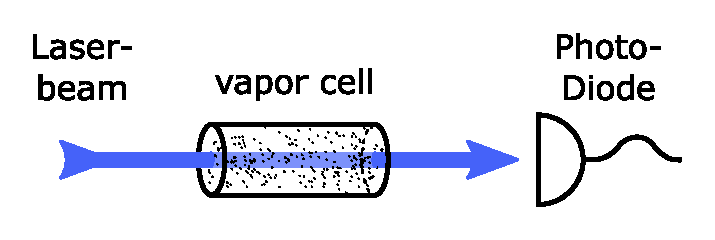
\includegraphics[width=0.35\textwidth]{absorption_spectroscopy_theory}    
    \caption{\label{fig:absorption_spectroscopy} Basic arrangement for ordinary 
        laser absorption spectroscopy.}
\end{wrapfigure}

The arrangement for ordinary laser absorption spectroscopy through a gaseous sample 
is shown in Fig.~\ref{fig:absorption_spectroscopy}. A laser beam passes through 
the vapor cell and its intensity is measured by a photodiode detector as the laser 
frequency \(\nu \) is scanned through the resonance frequency of an atomic transition. \\
To understand the absorption spectroscopy signal we will establish the basic 
equation describing how the laser intensity changes as it propagates through the 
sample. 
\pagebreak

%********************************** % Forth Section  **************************************
\section{Equation} %Section - 2.4
When a laser beam propagates through a gaseous sample only absorption and stimulated
emission change the intensity \(I\) of the laser beam and at the same time affect 
the proportion of the atoms in the ground \(P_0\) and exited state \(P_1\). 
Therefore the intensity at \(x+\dd x\) equals the intensity at \(x\) reduced by 
the missing intensity due to absorption and increased by the intensity due to 
stimulated emission. Each time there is an absorption process the atom absorbs 
the energy \(h\nu \) from the beam. The rate of absorption is defined by 
\(\alpha I \), so the power dissipated by one atom is \(\alpha I \cdot h\nu \). The number \(N\) of interacting
atoms with the beam is the atom density \(n_0\) multiplied by the considered volume
\(V = A \cdot \dd x \) where A is the beam cross section. Only the proportion of atoms in the 
ground state can contribute to the decrease in intensity, so the dissipated power
by absorption is
\begin{align}
    \alpha~I(x) ~ h\nu ~ n_0 ~ A ~ \dd x ~ P_0 ~ 
\end{align}
where \(P_0\) is the proportion of atoms in the ground state.
With the definition of \( intensity = \frac{power}{area}\) one obtains the dissipated
intensity by absorption 
\begin{align}
    \alpha~I(x) ~ h\nu ~ n_0 ~ P_0 ~ \dd x ~. 
\end{align}
Similarly for the stimulated emission the produced intensity is
\begin{align}
    \alpha~I(x) ~ h\nu ~ n_0 ~ P_1 ~ \dd x ~, 
\end{align}
where \(P_1\) is the proportion of atoms in the excited state and \(P_0+P_1 = 1\).
The variation of the laser intensity from \(x\) to
\(x+\dd x\) in the sample is as follows:
\begin{align} \label{eq:Int}
    I(x+\mathrm{d}x)-I(x) = - \alpha~I(x) ~ h\nu ~ n_0 ~ (P_0-P_1)~\mathrm{d}x 
\end{align}
This leads to the differential equation
\begin{align}\label{eq:diff_eq}
    \frac{ \mathrm{d}I }{ \mathrm{d}x } = -\kappa ~ I
\end{align}
where the \textit{absorption coefficient} (fractional absorption per unit of length)
\begin{align}\label{eq:kappa}
    \kappa = \alpha ~ h\nu  ~ n_0 ~ (P_0-P_1)~.
\end{align}

It should be noted that the proportionality to \(P_0-P_1 \) arises from the 
competition between stimulated emission and absorption and it is important to 
appreciate the consequences. If there are equal numbers of atoms in the ground 
and excited state (\(P_0-P_1=0\)), laser photons are as likely to be emitted by 
an atom in the excited state as they are to be absorbed by an atom in the ground 
state and there will be no attenuation of the incident beam. The attenuation 
maximizes when all atoms are in the ground state (\(P_0-P_1=1\)) because only 
absorption is possible. And the attenuation can even reverse sign (become an 
amplification as it does in laser gain media) if there are more atoms in the 
excited state (\(P_0>P_1\)).

%********************************** % Fifth Section  *************************************
\section{Doppler shifts}  %Section - 2.5

Atoms in a vapor cell move randomly in all three directions with a velocity 
distribution dependent on the temperature. Only the component of velocity parallel 
to the laser beam direction will be important when taking into account Doppler 
shifts and it is this component we refer to with the symbol \(v \). The density 
of atoms \(\dd n \) in having a velocity comprised between \(v \) and \(v+\dd v \) 
is given by the Boltzmann velocity distribution:
\begin{align}
    \dd n = n_0 ~ \sqrt{ \frac{m}{2\pi~k_B T} }~
    \exp{ \left( -\frac{m~v^2}{2~k_B T} \right ) }~\dd v
\end{align}
defining the standard deviation
\begin{align}
    \sigma_v = \sqrt{\frac{k_B T}{m}}
\end{align}
It can be rewritten using the canonical form of a Gaussian distribution
\begin{align}
    \dd n = n_0~\frac{1}{\sqrt{2\pi}~\sigma_v}~
    \exp{ \left( -\frac{v^2}{2~{\sigma_v}^2} \right ) }~\dd v
\end{align}
with a mean of zero~--~indicating the atoms are equally likely to be going in the
positive or negative \(z \) direction, i.e.\ they have positive or negative 
velocities. It is properly normalized so that the integral over all velocities 
(\(-\infty \rightarrow \infty) \) is \(n_0 \), the overall atom density. \\
Atoms moving with a velocity \(v \) see the laser beam Doppler shifted by the 
amount \(\nu~\frac{v}{c} \). This corresponds to a Doppler shifted resonance frequency
\begin{align}\label{eq:nu_shift}
    \nu'_0 = \nu_0 \left ( 1 + \frac{v}{c} \right)
\end{align}
in the lab frame. The sign has been chosen for a laser beam propagating in the 
positive direction so that the resonance frequency is blue shifted to higher 
frequencies if \(v \) is positive and red shifted if \(v \) is negative.\\
The absorption coefficient \(\dd\kappa \) from a velocity group \(\dd n \) at a 
laser frequency \(\nu \) is then obtained from Eq.~\ref{eq:kappa} by substituting 
\(\dd n \) for \(n_0 \) and by adjusting the Lorentzian dependence of \(\alpha \) 
so that it is centered on the Doppler shifted resonance frequency \(\nu'_0 \) 
(Eq.~\ref{eq:nu_shift}).
\begin{align}
    \dd\kappa = \alpha_0 ~ h\nu ~ (P_0-P_1) ~ \mathcal{L}(\nu,\nu'_0)~\dd n
\end{align}
The absorption coefficient from all atoms is then found by integrating over all 
velocity classes.

%********************************** % Sixth Section  *************************************
\section{\label{sec:weakfield}Absorption coefficient~-~weak field}   %Section - 2.6

We consider the weak-laser intensity case, where we have a very low intensity compared to 
\(I_\mathrm{s}\) and therefore nearly all atoms will be in the ground state, i.e., 
\(P_0-P_1 = 1 \) so that
\begin{align}
    \mathrm{d}\kappa = \alpha_0 ~ h\nu ~ n_0~\frac{1}{\sqrt{2\pi}~\sigma_v} ~
    \mathcal{L}(\nu,\nu'_0)~\exp{ \left( -\frac{v^2}{2 {\sigma_v}^2} \right ) }~
    \dd v
\end{align}
and
\begin{align}
    \kappa = \underbrace{ \alpha_0 ~ h\nu ~ n_0 ~ \frac{1}{\sqrt{2\pi}\sigma_v} }_{\beta} 
    \int\limits_{-\infty}^{\infty} 
    \frac{1}{ 1+4~{\left [\nu-\nu_0\left ( 1 + \frac{v}{c} \right) \right] }^2 / {\Gamma_\nu}^2 }~ 
    \exp{ \left (-\frac{v^2}{ 2~ {\sigma_v}^2 }\right ) }~\dd v
\end{align}
After the variable transformation
\begin{align*}
\left |~
    \begin{aligned}
        \nu'_0 =&~\nu_0\left ( 1+ \frac{v}{c} \right) \\
        v =&\left ( \frac{\nu'_0}{\nu_0} - 1 \right) c \\
        \dd v =&~\frac{c}{\nu_0}~\dd \nu'_0
    \end{aligned}
    ~\right |~ = \beta~\frac{c}{\nu_0} \int\limits_{-\infty}^{\infty} 
    \frac{1}{ 1+4~{(\nu-\nu'_0)}^2 / {\Gamma_\nu}^2 }~ 
    \exp{ \left ( -\frac{{(\nu'_0 - \nu_0)}^2~c^2 }{2~{\nu_0}^2~{\sigma_v}^2 } \right )}~
    \dd \nu'_0
\end{align*} 

and substitution \(\sigma_\nu = \frac{\nu_0}{c}~\sigma_v \) we get
\begin{align}
    \kappa = \beta~\frac{c}{\nu_0} \int\limits_{-\infty}^{\infty} 
    \frac{1}{ 1+4~{(\nu-\nu'_0)}^2 / {\Gamma_\nu}^2 }~ 
\exp{ \left ( -\frac{{(\nu'_0 - \nu_0)}^2 }{2~{\sigma_\nu}^2 } \right )}~\dd \nu'_0 
\label{eq:intlorgau}
\end{align}
Now we compare the width parameters from the Lorentzian (see table~\ref{table:iso_prop}) 
with the Gaussian function and at room temperature (\SI{20}{\degreeCelsius}) (see
Fig.~\ref{fig:gauvslor}):

\begin{minipage}[c][][c]{.45\textwidth}
\centering
\begin{align*}
    &\sigma_\nu = \frac{c}{\lambda_\mathrm{D2}}~\sqrt{\frac{k_B T}{m_{Rb85}~c^2}} 
    \approx \SI{403}{\mega\hertz} \\ \\
    &\Gamma_{\nu,\mathrm{D2}} = \SI{0.282}{\mega\hertz} \\ \\
    &\Rightarrow \Gamma_{\nu,\mathrm{D2}} \ll \sigma_\nu
\end{align*}
\end{minipage}
\hfill
\begin{minipage}[c]{.45\textwidth}
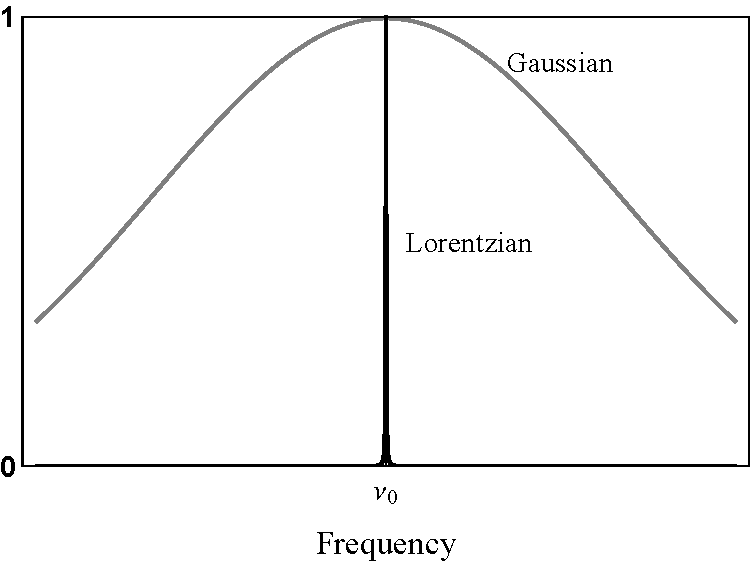
\includegraphics[width=\textwidth]{gauvslor}
\captionof{figure}{\label{fig:gauvslor} The Lorentzian compared to the Gaussian profile}
\end{minipage}
\bigskip

As we can see the Lorentzian function is significantly different from zero only 
within a very narrow range. Consequently the Gaussian remains relatively constant 
over the width of \(\Gamma_{\nu,\mathrm{D2}} \). Therefore Eq.~(\ref{eq:intlorgau}) 
can be accurately determined as the integral of the Lorentzian times the 
value of the exponential at \(\nu'_0 = \nu \):
\begin{align}
    = \beta~\frac{c}{\nu_0}~
    \exp{ \left ( -\frac{{(\nu - \nu_0)}^2 }{2~{\sigma_\nu}^2 } \right )} 
    \int\limits_{-\infty}^{\infty} \frac{1}{ 1+4~{(\nu-\nu'_0)}^2 / {\Gamma_\nu}^2 }~
    \dd \nu'_0
\end{align}
and with the solution of the Lorentzian integral
\begin{align}
    \int\limits_{-\infty}^{\infty} \mathcal{L}(\nu,\nu'_0)~\dd \nu'_0 = 
    \frac{\pi~\Gamma_\nu}{2}
\end{align}
we finally get the absorption coefficient in a weak field
\begin{align}\label{eq:kappa_weakfield}
    \kappa = \kappa_0~\exp{ \left ( -\frac{{(\nu - \nu_0)}^2 }{2~{\sigma_\nu}^2 } \right )}
     ~~\text{with}~~ \kappa_0 = \alpha_0 ~ h\nu ~ n_0 ~ \frac{1}{\sqrt{2\pi}~\sigma_\nu}~
     \frac{\pi~\Gamma_\nu}{2}
\end{align}


%********************************** % Seventh Section  *************************************
\section{Population}   %Section - 2.7

To determine the general case of the absorption coefficient we need to determine 
\(P_0-P_1 \). For that we have to take into account the changes to the ground and 
excited state populations arising from a laser beam propagating through the cell. 
The rate equations for the ground and excited state are therefore:
\begin{align}
    \frac{\mathrm{d}P_0}{\mathrm{d}t} &= \Gamma_{\omega,tot} P_1 - \alpha~I (P_0-P_1) \nonumber \\
    \frac{\mathrm{d}P_1}{\mathrm{d}t} &= -\Gamma_{\omega,tot} P_1 + \alpha~I (P_0-P_1)
\end{align} 
where the first term on the right in each equation arises from spontaneous emission 
and the second term arises from absorption and stimulated emission.\\
With the additional equation \(P_0+P_1=1 \) and the steady state condition
\begin{align}
    \frac{\mathrm{d}P_0}{\mathrm{d}t} = \frac{\mathrm{d}P_1}{\mathrm{d}t} = 0
\end{align}
we get for the populations
\begin{align}
        P_0 = \frac{\Gamma_{\omega,tot} + \alpha~I}{\Gamma_{\omega,tot} + 2 \alpha~I}~; 
        \qquad 
        P_1 = \frac{\alpha~I}{\Gamma_{\omega,tot} + 2 \alpha~I}
\end{align}
which leads to
\begin{align}
    (P_0-P_1) = \frac{\Gamma_{\omega,tot}}{\Gamma_{\omega,tot} + 2 \alpha~I} 
\end{align}
As we can see the population difference is dependent on \(\Gamma_{\omega,tot} \) 
(spontaneous decay rate), which is related to the \textit{Lorentzian width parameter}. 
To combine the Lorentzians in \(\alpha \) (Eq.~\ref{eq:alpha}) and \( (P_0-P_1) \) 
we will define \(\Delta\nu = 2~(\nu-\nu_0) \):
\begin{align}
    \alpha = \alpha_0~\frac{1}{ 1+ \Delta\nu^2 / {\Gamma_\nu}^2 } 
    = \alpha_0~\frac{\Gamma_\nu^2}{\Gamma_\nu^2 + \Delta\nu^2}~; \qquad
    (P_0-P_1) = \frac{2\pi~\Gamma_{\nu,tot}}{2\pi~\Gamma_{\nu,tot} + 2 \alpha~I}
\end{align}
and get
\begin{align}
    (P_0-P_1)\alpha = \frac{2\pi~\Gamma_{\nu,tot}}
    {2\pi~\Gamma_{\nu,tot} + 2I~\alpha_0~\frac{\Gamma_\nu^2}{\Gamma_\nu^2 + \Delta\nu^2}}~ 
    \alpha_0~\frac{\Gamma_\nu^2}{\Gamma_\nu^2 + \Delta\nu^2} = 
    \frac{\alpha_0~\pi~\Gamma_\nu^2~\Gamma_{\nu,tot}}
    {\pi~\Gamma_{\nu,tot}~(\Gamma_\nu^2 + \Delta\nu^2)+I~\alpha_0~\Gamma_\nu^2}
\end{align}
dividing with \(\pi~\Gamma_\nu \) and substitute in the denominator \(\alpha_0 \) 
with the definition of Eq.~\eqref{eq:gamma_relation} and~\eqref{eq:saturationInt} 
leads to
\begin{align}
    (P_0-P_1)\alpha = \alpha_0~\frac{1}
    {1 + \frac{\Delta\nu^2}{\Gamma_\nu} + \frac{2I}{I_s}\frac{\Gamma_\nu}{\Gamma_{\nu,tot}} } 
    = \frac{\alpha_0}{(1 + \frac{2I}{I_s}\frac{\Gamma_\nu}{\Gamma_{\nu,tot}})}~
    \frac{1}{1+ \frac{\Delta\nu^2}
    {\Gamma_\nu^2 \left(1 + \frac{2I}{I_s}~\frac{\Gamma_\nu}{\Gamma_{\nu,tot}} \right)}}
\end{align}
and with the definition of the power-broadened \textit{width parameter}
\begin{align}
    \Gamma'_\nu = \Gamma_\nu \sqrt{1 + \frac{2I}{I_s}~\frac{\Gamma_\nu}{\Gamma_{\nu,tot}} }
\end{align}
we obtain
\begin{align}\label{eq:kappa_weak}
    (P_0-P_1)\alpha = 
    \frac{\alpha_0}{ \left( 1 + \frac{2I}{I_s}\frac{\Gamma_\nu}{\Gamma_{\nu,tot}} \right )}~
    \mathcal{L}'(\nu,\nu_0)~~\text{and}~~\mathcal{L}'(\nu,\nu_0)= 
    \frac{1}{1+ \frac{{4~(\nu-\nu_0)}^2}{{\Gamma'_\nu}^2}}
\end{align}

%********************************** % Eighth Section  *************************************
\section{Absorption coefficient~-~general case}  %Section - 2.8

For the general case we take now into account the velocity groups and their 
corresponding Doppler shifts for the case \(P_0-P_1 \neq 1 \) and therefore 

\begin{align}
    \mathrm{d}\kappa = 
    h\nu~n_0~\frac{\alpha_0}{(1 + \frac{2I}{I_s}~\frac{\Gamma_\nu}{\Gamma_{\nu,tot}})} 
    \frac{1}{\sqrt{2\pi}~\sigma_v} \mathcal{L}'(\nu,\nu'_0) 
    \exp{ \left( -\frac{v^2}{2~{\sigma_v}^2} \right ) } \dd v
\end{align}
and
\begin{align}
    \kappa = h\nu~n_0~\frac{\alpha_0}{(1 + \frac{2I}{I_s}~\frac{\Gamma_\nu}{\Gamma_{\nu,tot}})}~ 
    \frac{1}{\sqrt{2\pi}~\sigma_v} 
    \int\limits_{-\infty}^{\infty} 
    \frac{1}{ 1+4~{\left [\nu-\nu_0\left ( 1 + \frac{v}{c} \right) \right] }^2 / {\Gamma'_\nu}^2 } 
    \exp{ \left (-\frac{v^2}{ 2~{\sigma_v}^2 }\right ) } \dd v
\end{align}
The calculation can be performed as in Section~\ref{sec:weakfield} with the only 
addition of the the power-broadened \textit{width parameter} \(\Gamma'_\nu \). 
This leads to
\begin{align}
    \kappa &= h\nu~n_0~
    \frac{\alpha_0}{(1 + \frac{2I}{I_s}~\frac{\Gamma_\nu}{\Gamma_{\nu,tot}})}~ 
    \frac{1}{\sqrt{2\pi}~\sigma_\nu}~\frac{\pi~\Gamma'_\nu}{2}~
    \exp{ \left ( -\frac{{(\nu - \nu_0)}^2 }{2~{\sigma_\nu}^2 } \right )} \nonumber \\
    &= \frac{\kappa_0}{\sqrt{1 + \frac{2I}{I_s}~\frac{\Gamma_\nu}{\Gamma_{\nu,tot}}}}~
    \exp{ \left ( -\frac{{(\nu - \nu_0)}^2 }{2~{\sigma_\nu}^2 } \right )}
\end{align}
and subsequently
\begin{align}
    \kappa = \kappa'_0~\exp{ \left ( -\frac{{(\nu - \nu_0)}^2 }{2~{\sigma_\nu}^2 } \right )}
    ~~\text{with}~~ \kappa'_0 = 
    \frac{\kappa_0}{\sqrt{1 + \frac{2I}{I_s}~\frac{\Gamma_\nu}{\Gamma_{\nu,tot}}}}~.
    \label{eq:kappa_final}
\end{align}


%********************************** % Ninth Section  *************************************
\section{Beer-Lambert Law}  %Section - 2.9
As derived before (Eq.~\ref{eq:kappa_final}) \(\kappa \) is dependent on the 
intensity, so solving Equation~\ref{eq:diff_eq} is not an easy task. But in the 
case of low intensity we can make an assumption that \(\kappa \) is independent
from \(I\). The solution of the differential equation is then:
\begin{align}\label{eq:beer_lambert}
   I(x)=I_0~\mathrm{e}^{-\kappa x}~.
\end{align}
This solution is called \textit{Beer-Lambert law} and will be used in Chapter 4 
as basis for our evaluation.
\pagebreak


%********************************** % Tenth Section  *************************************
\section{Real Rb atom D2 line levelscheme}\label{sec:realrubidium} %Section - 2.10

\begin{figure}[ht]
    \centering
    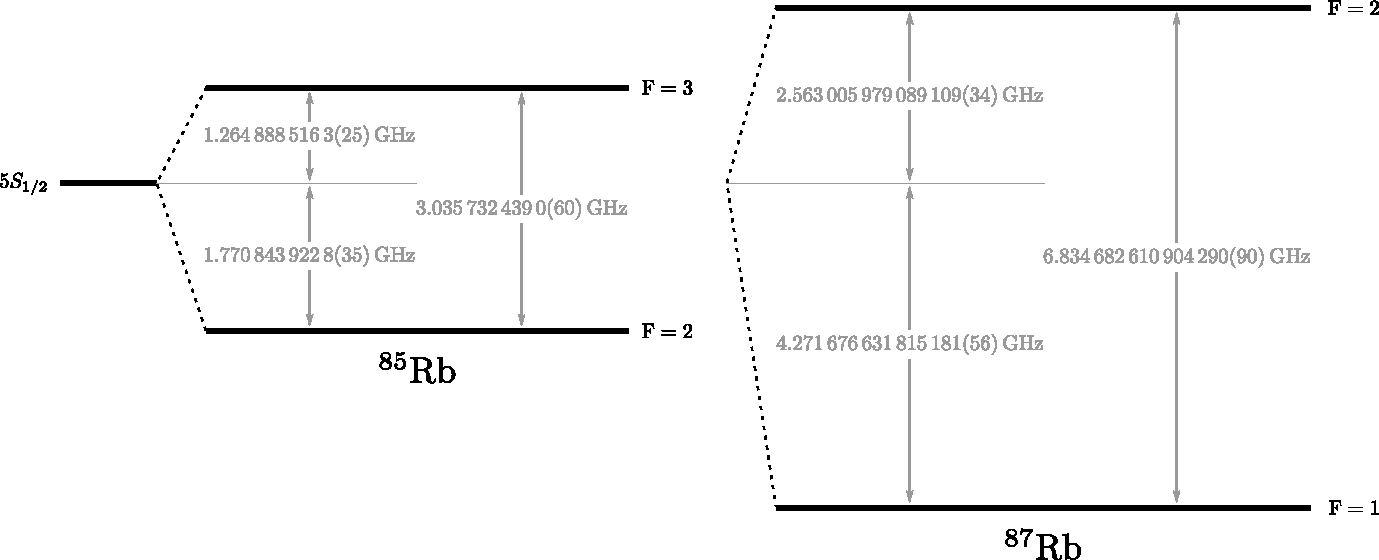
\includegraphics[width=0.95\textwidth]{hyperfine_scheme}
    \caption{\(5^{2}S_{1/2} \) hyperfine structure of \(^{85}\)Rb 
    and \(^{87}\)Rb.}    
\end{figure}

The transition of interest is, as we have discussed before, the \(5^{2}S_{1/2} 
\rightarrow 6^{2}P_{3/2}\) of rubidium. In the cell we use, two isotopes of Rb 
are present: \(^{85}\)Rb and \(^{87}\)Rb.
As we can see both isotopes have the same transition energy, but due to the 
different spin I (see table:~\ref{table:iso_prop}) the hyperfine energy splitting
is different \citep{nist_asd}: \SI{3}{\giga\hertz} for \(^{85}\)Rb and 
\SI{6.8}{\giga\hertz} for \(^{87}\)Rb. This is the reason why we witness four 
Doppler peaks in our spectrum when performing a spectroscopy (see Fig.~\ref{fig:doppler}). 
The different amplitudes between the two isotopes are explained through their 
abundance in the cell, \SI{72.2}{\percent} for \(^{85}\)Rb and \SI{27.8}{\percent} 
for \(^{87}\)Rb. And the cause for the difference among one isotope is that the 
different hyperfine states, e.g.~\(F=2\) and \(F=3\) for \(^{85}\)Rb, have 
\(m_F = 2F+1 \) distinct levels. The thermal energy at \SI{300}{\kelvin} is 
three orders in magnitude higher than the hyperfine splitting and thus each of 
the \(m_F\) levels are equally populated.  

\begin{figure}[h]
\centering
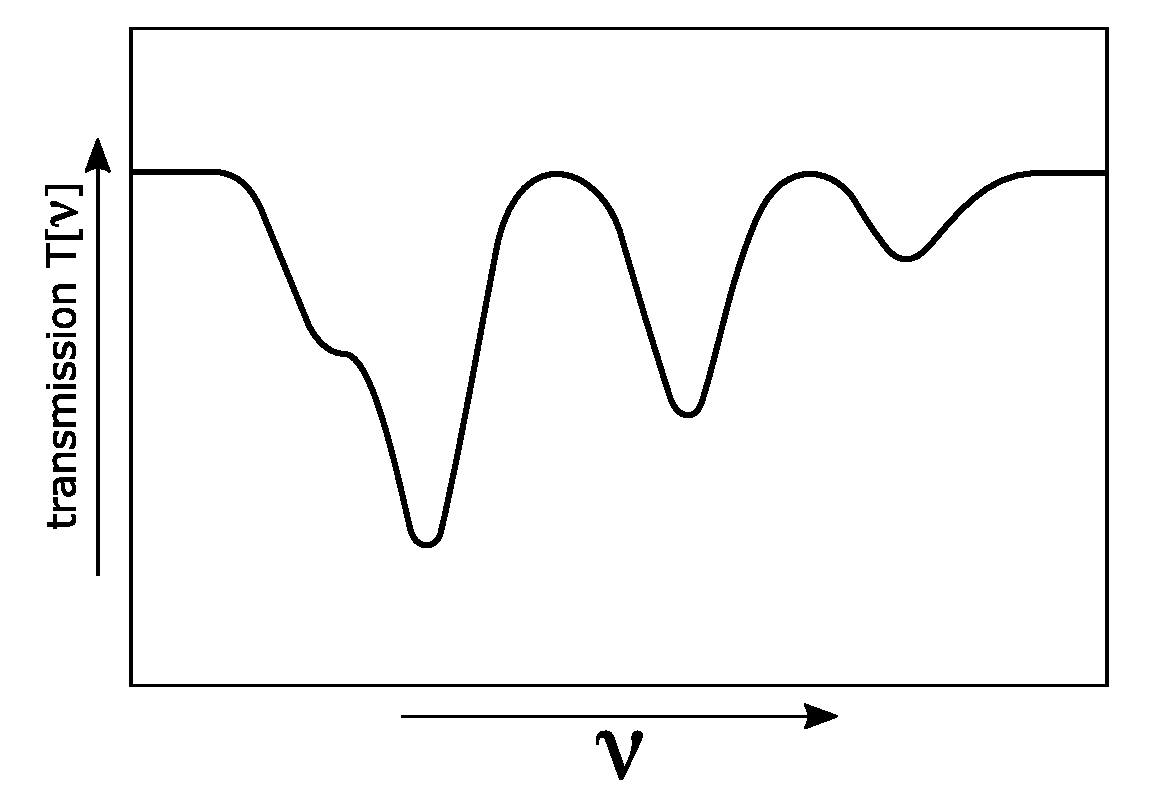
\includegraphics[width=0.5\textwidth]{spectrum_doppler}
\caption{\label{fig:doppler}Doppler spectrum of D2 line} 
\end{figure}

\pagebreak
%********************************** % Eleventh Section  **********************************
\section{Rubidium data}  %Section - 2.11

\begin{table}[h]
\centering
\begin{tabular*}{0.9\textwidth}{@{\extracolsep{\fill} }l l c c}
\toprule
& & \multicolumn{2}{c}{Rubidium} \\
\midrule
Isotope & [1] & 85 & 87 \\
Atomic mass & [\si{\atomicmassunit}] & 84.911794 & 86.909187 \\
\num{e-25} & [\si{\kilogram}] & 1.40999 & 1.44316 \\
Abundance & [\si{\percent}] & 72.17 & 27.83 \\
Spin I & [1] & \(\sfrac{5}{2}\) & \(\sfrac{3}{2}\) \\
Lifetime \(6^{2}P_{3/2}\) & \([ \si{\nano\second} ]\) & & \num{112} \\
Lifetime \(6^{2}P_{1/2}\) & \([ \si{\nano\second} ]\) & & \num{125} \\
Wavelength D1-Line (\(6^{2}P_{1/2} \rightarrow 5^{2}S_{1/2}\)) & [\si{\nano\meter}] & 421.5524 & \\
Wavelength D2-Line (\(6^{2}P_{3/2} \rightarrow 5^{2}S_{1/2}\)) & [\si{\nano\meter}] & 420.1792 & \\
A\(_{\mathrm{ki,D1}},~\Gamma_{\omega,\mathrm{D1}}\) @ \SI{421}{\nano\meter} & \([ \si{\per\second} ] \) & \num{1.50e6} & \\
A\(_{\mathrm{ki,D2}},~\Gamma_{\omega,\mathrm{D2}}\) @ \SI{420}{\nano\meter} & \([ \si{\per\second} ] \) & \num{1.77e6} & \\
Natural linewidth \(\Gamma_{\nu,\mathrm{D1}}\) & \([ \si{\mega\hertz} ]\) & \num{0.239} & \\
Natural linewidth \(\Gamma_{\nu,\mathrm{D2}}\) & \([ \si{\mega\hertz} ]\) & \num{0.282} & \\
\bottomrule
\end{tabular*}
\caption{\label{table:iso_prop}Properties of rubidium isotopes}
\end{table}
\pagebreak



%!TEX root = ../thesis.tex
% Spellcheck ignore
% cSpell:ignore midskip, Teledyne, Lecroy,oscilloscope, piezo, smallskip, dialimitplot, FWHM, diaminplot, meanplot, diaplot, Irange, wavemeter, rbcell, centi, extracolsep, toprule, midrule, bottomrule, milli, eqref, detuning, photodiode, Toptica, photonics, nano, giga, collimated, bigskip, captionof, minipage, pagebreak, wincam, includegraphics,wrapfigure, ifpdf, graphicspath
%*******************************************************************************
%****************************** Third Chapter **********************************
%*******************************************************************************

\chapter{Experiment}

\ifpdf{}
    \graphicspath{{Chapter3/Figs/Raster/}{Chapter3/Figs/PDF/}{Chapter3/Figs/}}
\else
    \graphicspath{{Chapter3/Figs/Vector/}{Chapter3/Figs/}}
\fi

%********************************** % First Section  **************************************
\section{Laser} %Section - 3.1 

For all our measurements we used a \SI{420}{\nano\meter} DL (extended cavity laser
diode) pro HP laser with a 
DLC pro controller from Toptica photonics. An optical isolator (OI) is included
into the laser and thus the given powers are after OI\@.

\bigskip
\begin{table}[h]
    \centering
    \begin{tabular*}{0.6\textwidth}{@{\extracolsep{\fill} } l l}
    \toprule
    Specifications \\
    \midrule
    Wavelength: & \SI{421.0}{\nano\meter} \\
    Coarse Tuning: & \SI{419.5}{\nano\meter}~-~\SI{422.5}{\nano\meter} \\
    Max.~power: & \SI{78.0}{\milli\watt} \\
    At diode current: & \SI{93}{\milli\ampere} \\
    Mode Hop Free Tuning: & \SI{79}{\giga\hertz} at \SI{78.5}{\milli\ampere}\\
    \bottomrule
    \end{tabular*}
    \caption{\label{table:laser_spec} Specifications of Toptica DL pro HP 
    \SI{421}{\nano\meter}}
\end{table}

The laser has to be tuned to the right wavelength.
For that the beam was guided into a fiber and feeded into a wavemeter. The coarse 
tuning of the laser was done using the mechanical screw which changes the angle 
of the grating. Then the fine tuning was done playing both on the diode current
and the socket temperature on which the laser is mounted. To have a specific 
output power one would first adjust the diode current, which fines the power
and then readjust the temperature. \\
We characterized the beam profile \SI{50}{\centi\meter} after the beam outlet
(see Fig.~\ref{fig:beam50cm}), where we could see that the beam had a waist 
diameter of \(\approx\SI{933}{\micro\meter}\). It should be noted that the beam 
profile was not perfectly gaussian.

\begin{figure}
    \centering
    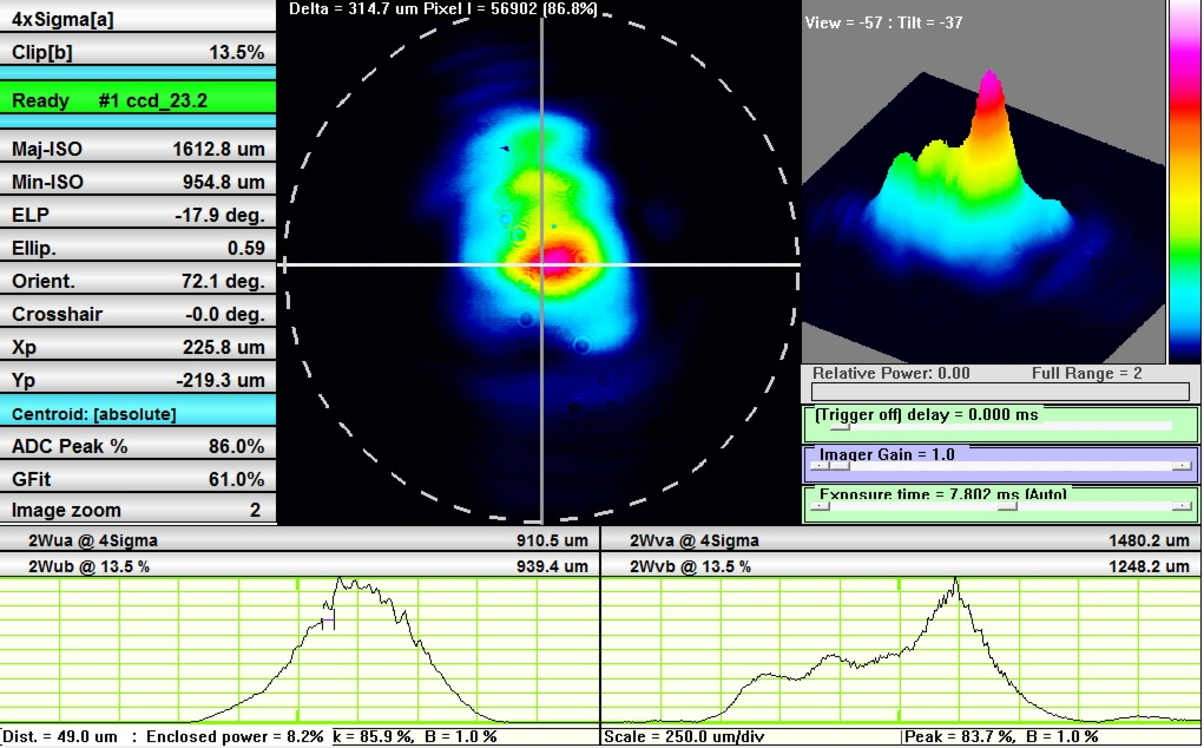
\includegraphics[width=.7\textwidth]{beam50cm}
    \caption{\label{fig:beam50cm} Beam profile after \SI{50}{\centi\meter}}
\end{figure}

%********************************** % Second Section  **************************************
\section{Setup} %Section - 3.2

\begin{figure}[H]
    \centering
    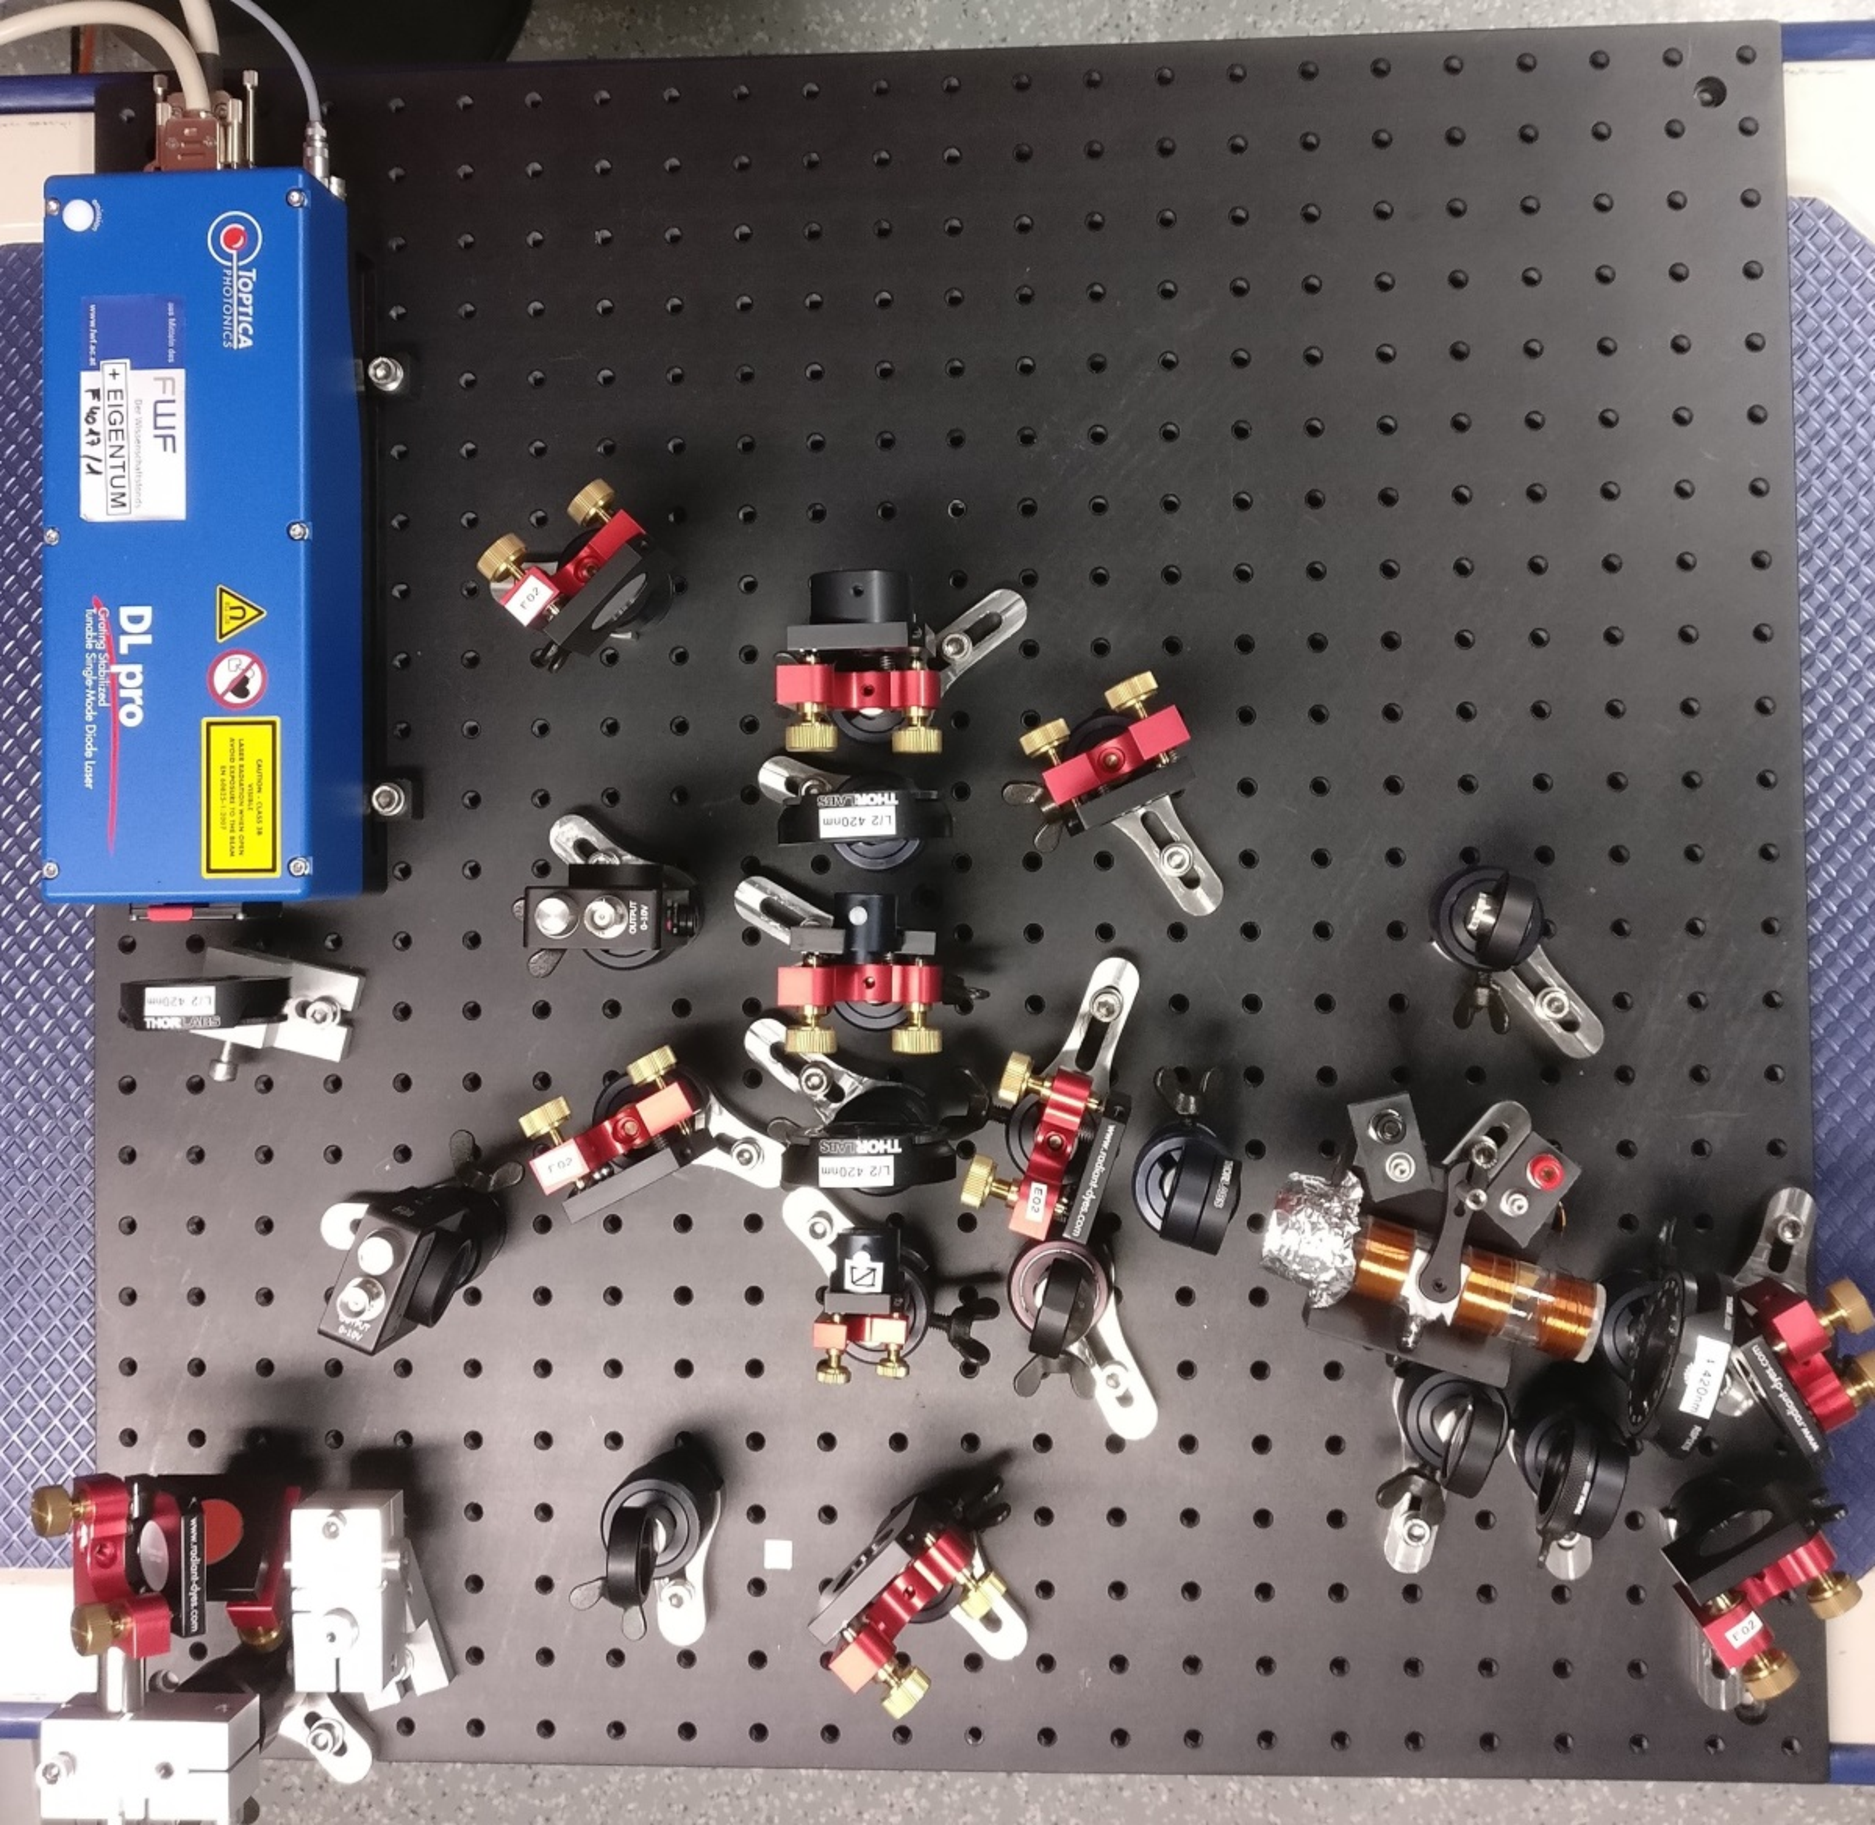
\includegraphics[width=.5\textwidth]{breadboard}
    \caption{\label{fig:breadboard} Setup mounted on a \(60 \times 60 \)\si{\centi\meter} 
    breadboard.}
\end{figure}

The laser bench should be placed on the experiment breadboard and thus, we took
into account space constraints when designing the beam path (see Fig.~\ref{fig:breadboard}).
The whole setup was mounted on a breadboard (\(60 \times 60 \)\si{\centi\meter}) 
and was divided into two parts via a polarization beam splitter (PBS) and a 
\(\lambda/2\) plate. Part of the beam power will be directed to the trap arm. 
This part was not built, we just placed a beam dump to block the beam, as can be 
seen in Fig.~\ref{fig:wincam_before}. But the occupied area had to be taken into 
account and we tried to built the spectroscopy setup (second arm) as compact as 
possible (see Fig.~\ref{fig:breadboard}).

\begin{figure}[H]
    \centering
    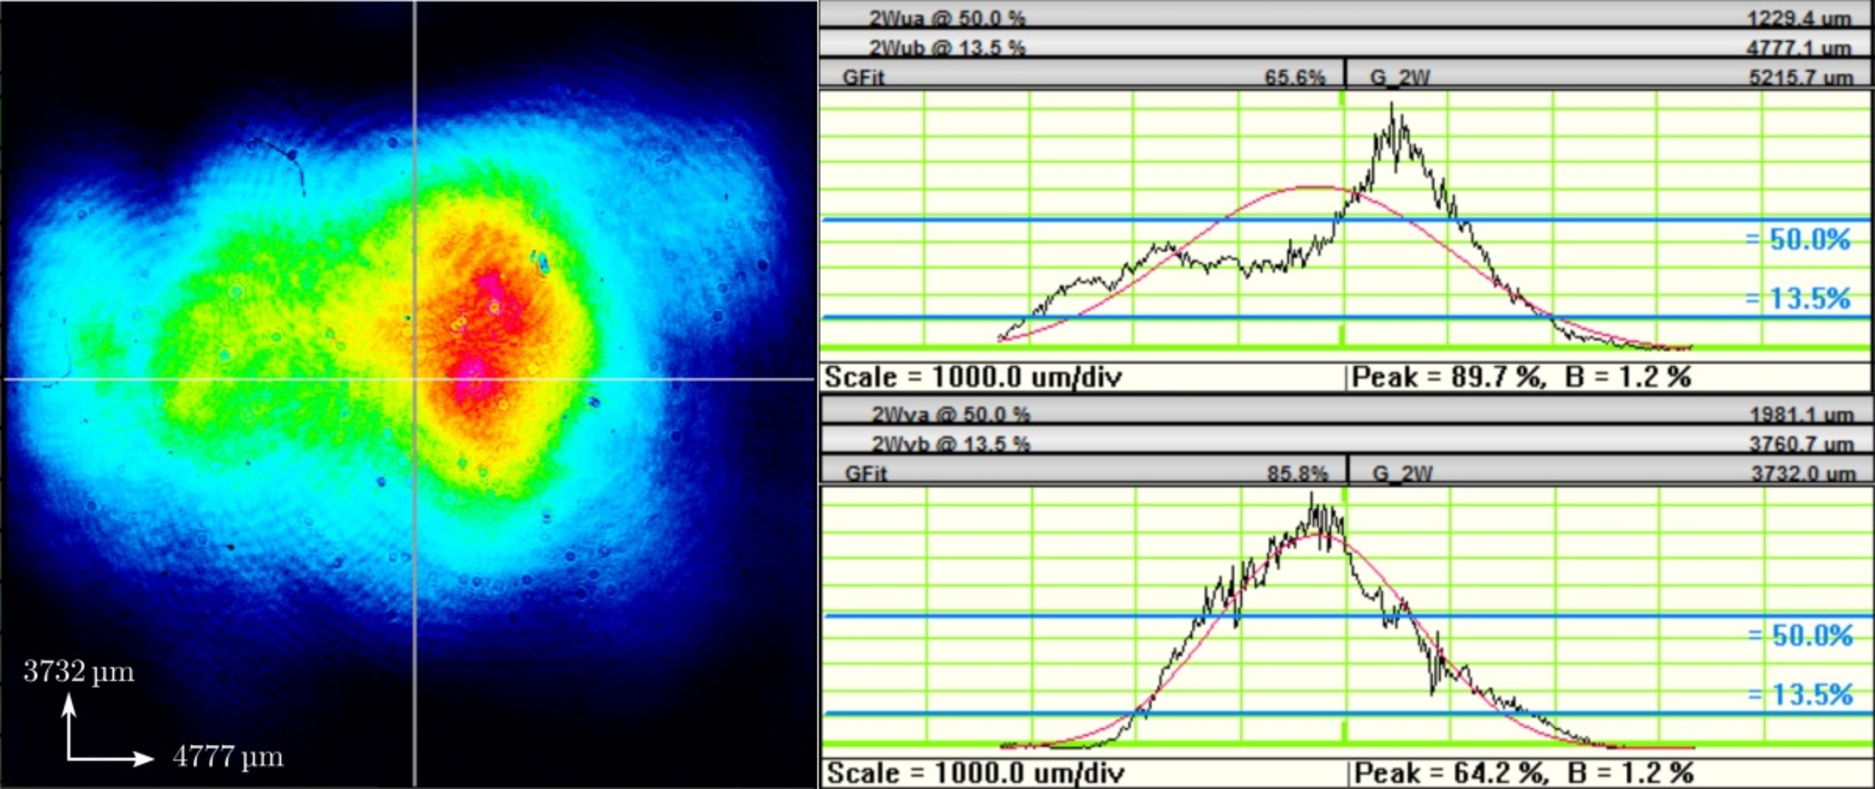
\includegraphics[width=0.7\textwidth]{beam_widened} 
    \caption{\label{fig:beam_widened} Beam profile after telescope setup.}
\end{figure}

We want to assume that all atoms receive the same intensity, such that we can 
use \(I = \frac{power}{cross~section} \). To achieve this, one has to change the 
beam profile by widening and additionally cropping to the center of the beam. 
To widen the beam we used a telescope setup after the PBS
with two lenses of different focal lengths (\(f_1 = \SI{2.5}{\centi\meter} 
\text{ and } f_2 = \SI{10}{\centi\meter}\)), which resulted in a beam with a waist
diameter of \(\approx \)\SI{3760}{\micro\meter} (see Fig.~\ref{fig:beam_widened}).
Therefore our magnification is \(\frac{3760}{933} = 4 = \frac{10}{2.5}\). Then 
the beam is cropped using an iris and guided through the cell with two mirrors. 
The iris aperture was chosen, in order to select the flat intensity.\\
The cell used in the setup is \SI{10}{\centi\meter} long and containing \(^{85}\)Rb
and \(^{87}\)Rb in isotopic concentrations. In order to increase absorption, we 
heated the rubidium cell with wire coils as seen in Fig.~\ref{fig:coils}. 
We used a wire with a diameter of \SI{0.315}{\milli\meter} for an higher resistance 
per unit of length. On the cell are four coils with \SI{35} turns each. The coils 
have alternating clock- and counter-clockwise windings, such that the generated 
magnetic fields cancel each other. The heater was operated with \SI{2}{\ampere} 
direct current to produce enough heat such that most of the condensed rubidium 
changed into the gas phase.

\begin{figure}[H]
    \centering
    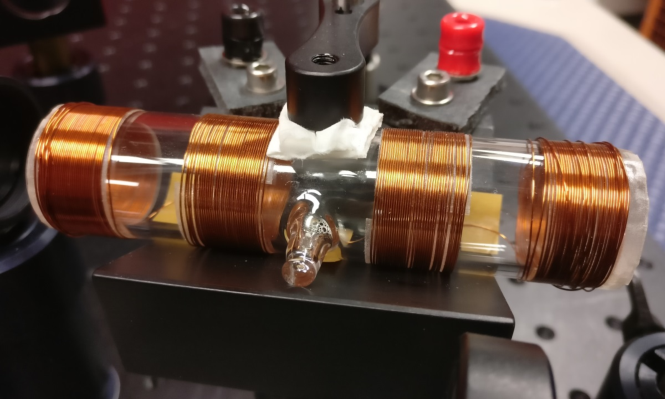
\includegraphics[width=.6\textwidth]{rbcell_coils}
    \caption{\label{fig:coils} Rubidium cell with applied copper wire coils for
    heating.}
\end{figure}


\pagebreak
%********************************** % Third Section  **************************************
\section{\label{sec:laser_dia_measurement}Laser diameter measurement} %Section - 3.3
\begin{minipage}[c]{.45\textwidth}
    \centering
    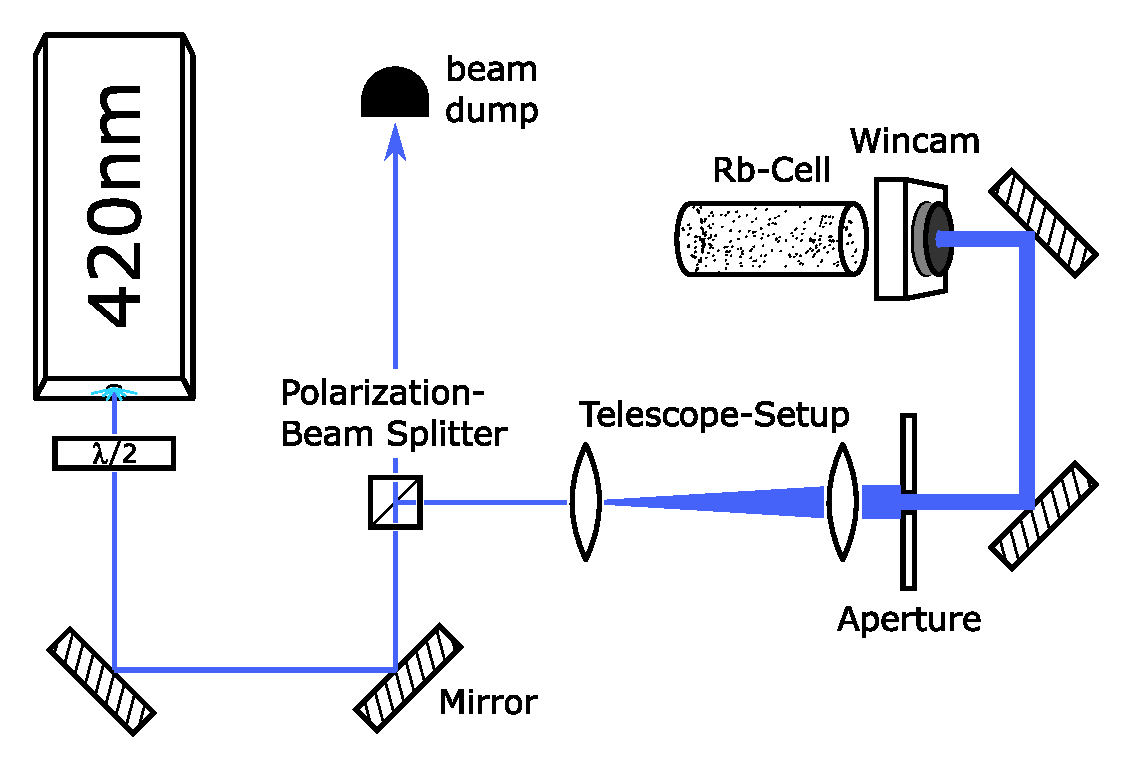
\includegraphics[width=.9\textwidth]{wincam_before}
    \captionof{figure}{\label{fig:wincam_before} Laser diameter measurement before 
    rubidium cell}
\end{minipage}
\hfill
\begin{minipage}[c]{.45\textwidth}
    \centering
    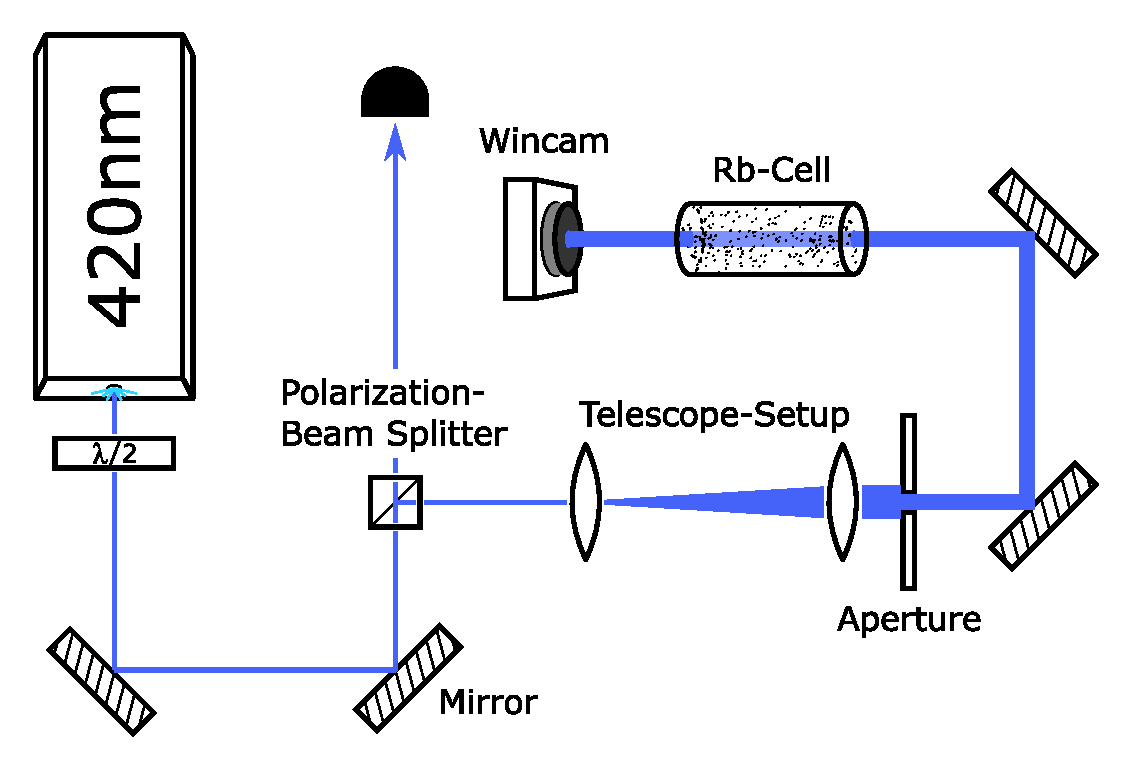
\includegraphics[width=.9\textwidth]{wincam_after}
    \captionof{figure}{\label{fig:wincam_after} Laser diameter measurement after 
    rubidium cell}
\end{minipage}

\begin{wrapfigure}{Hr}{.4\textwidth}
    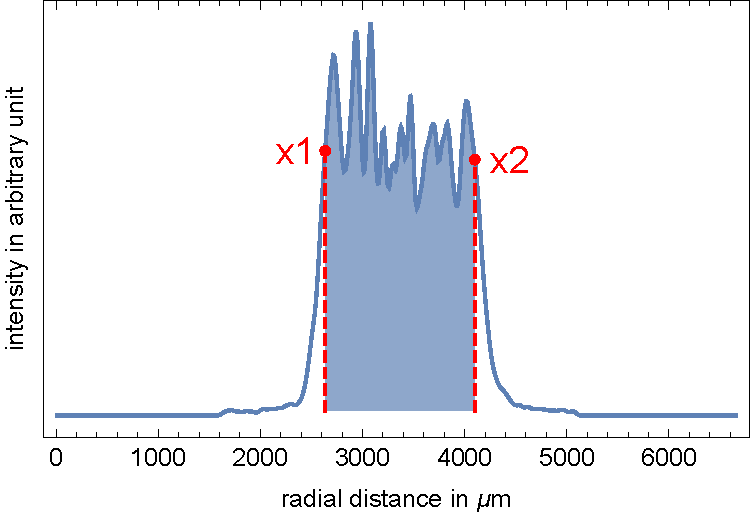
\includegraphics[width=0.33\textwidth]{dialimitplot}    
    \caption{\label{fig:diaminplot} By hand estimated beam limits.}
    \vspace{1em}
    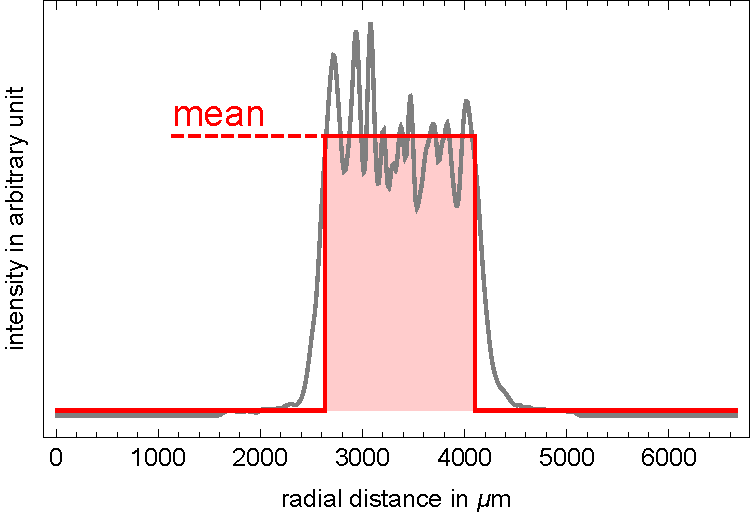
\includegraphics[width=0.33\textwidth]{meanplot}    
    \caption{\label{fig:meanplot} Equivalent flat hat beam.}
    \vspace{1em}
    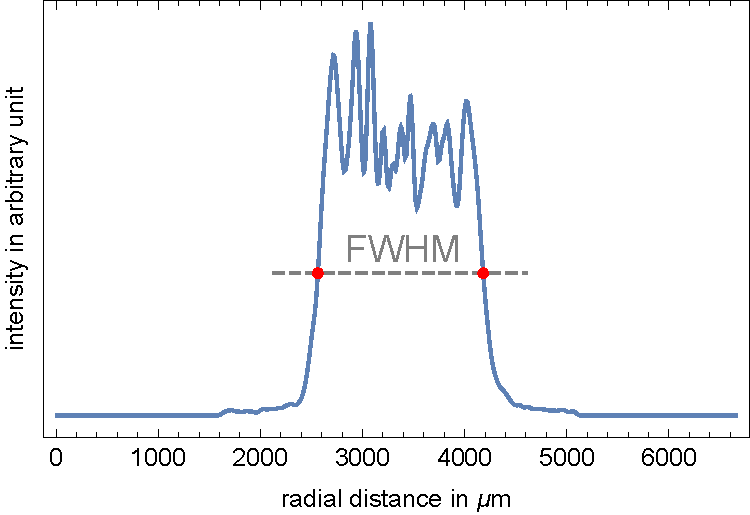
\includegraphics[width=0.33\textwidth]{diaplot}    
    \caption{\label{fig:diaplot} FWHM defines the estimated diameter.}
\end{wrapfigure}

\bigskip
In order to calculate the laser intensity one needs to measure the beam power and 
the beam cross section or rather the beam diameter. With a beam profiler (in our 
case a WinCamD) a measurement is performed in front and after the cell to measure 
and characterize the beam profile and check if the beam is collimated after the 
widening (see Fig.~\ref{fig:wincam_before}~and~\ref{fig:wincam_after}). 
The beam waist diameter calculated by the WinCamD application (see Fig.~\ref{fig:beam}) 
under the assumption of a gaussian beam is not correct. We will instead use a 
flat hat model for the evaluation and take the diameter where the power drops to 
half of the maximum power. It should be noted that the power is not constant over 
the whole beam profile, but shows \SI{30}{\percent} of fluctuations. We can then 
use the mean where the edge of the beam maximum is determined by hand. This leads 
to an uncertainty of \SI{+-100}{\micro\meter} per measurement. To obtain the 
equivalent flat hat intensity one has to integrate over the plot from limit to 
limit and divide by the interval (see Fig.~\ref{fig:meanplot}). The diameter of 
the beam is defined by its FWHM, this would be half the mean intensity as seen 
in Fig.~\ref{fig:diaplot}. The estimated beam diameter before the cell calculated 
out of the x- and y-axis slice is \SI[separate-uncertainty]{1608+-70}{\micro\meter} 
and \SI[separate-uncertainty]{1649+-70}{\micro\meter} after the cell. Therefore
the mean diameter is \SI[separate-uncertainty]{1628+-50}{\micro\meter} which
leads to an estimated cross section of
\SI[separate-uncertainty]{2.083+-0.128e-6}{\meter\squared}.


\pagebreak
\begin{figure}
    \centering
    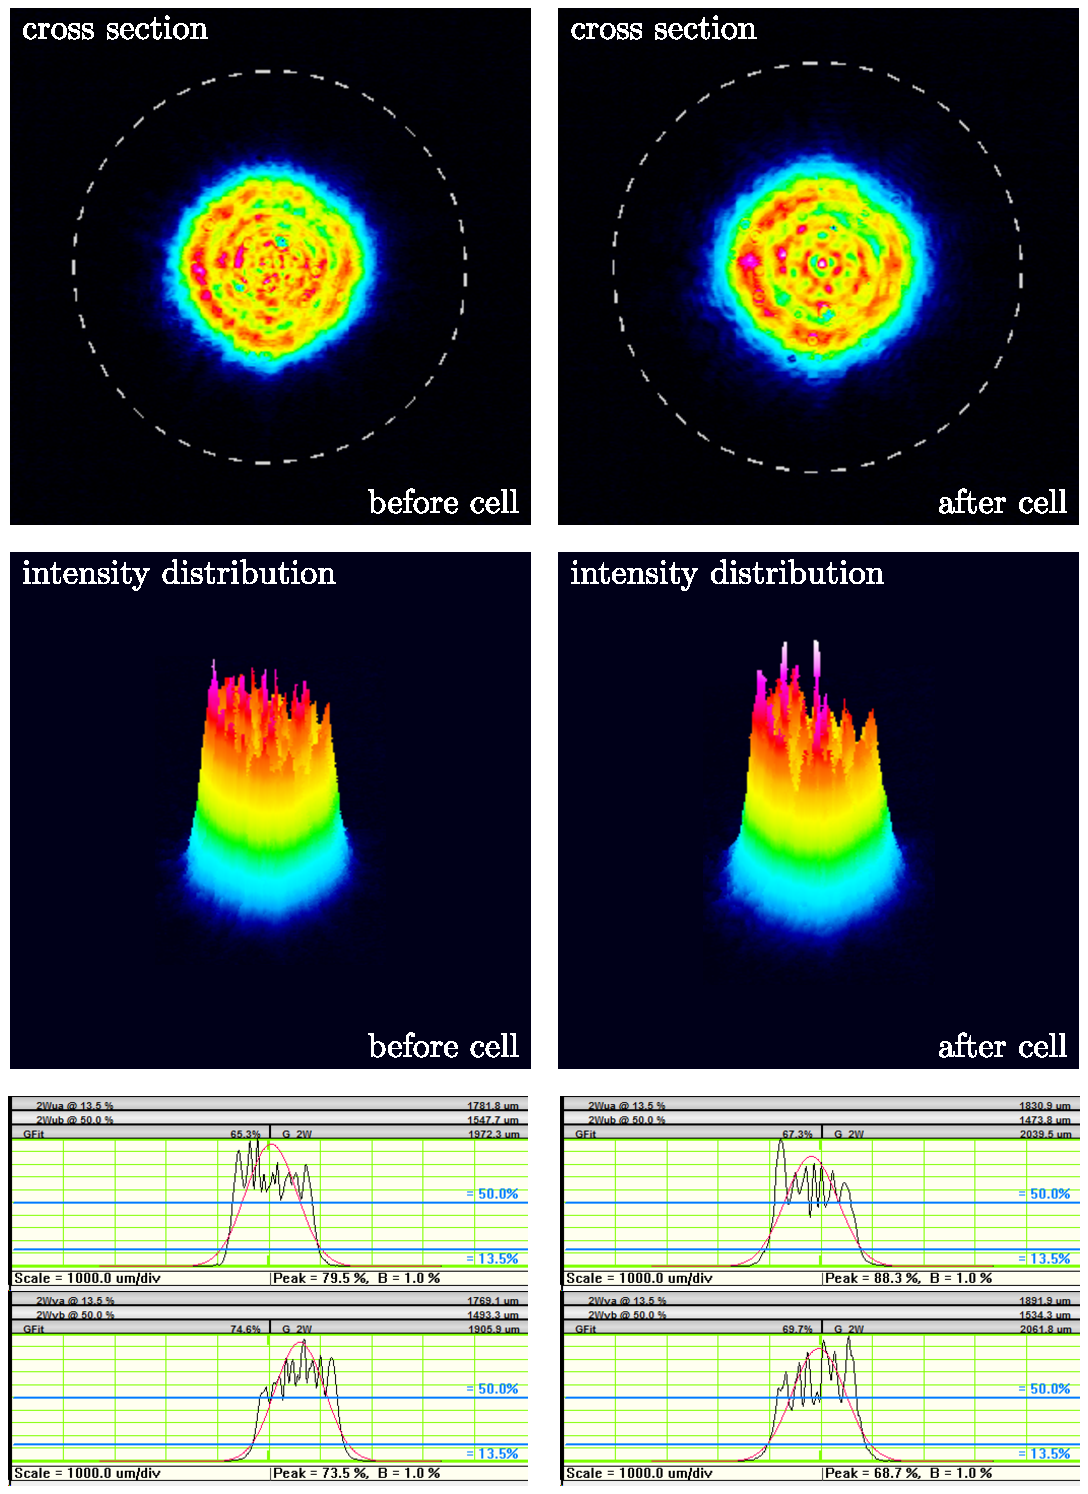
\includegraphics[width=.9\textwidth]{beam}
    \caption{\label{fig:beam} Cross section, intensity distribution and x- and 
    y-axes slices through beam center before and after cell transit.}
\end{figure}

\pagebreak
%********************************** % Forth Section  *************************************
\section{Absorption spectroscopy}\label{sec:absorption_spec} %Section - 3.4

\begin{figure}[!htb]
    \centering
    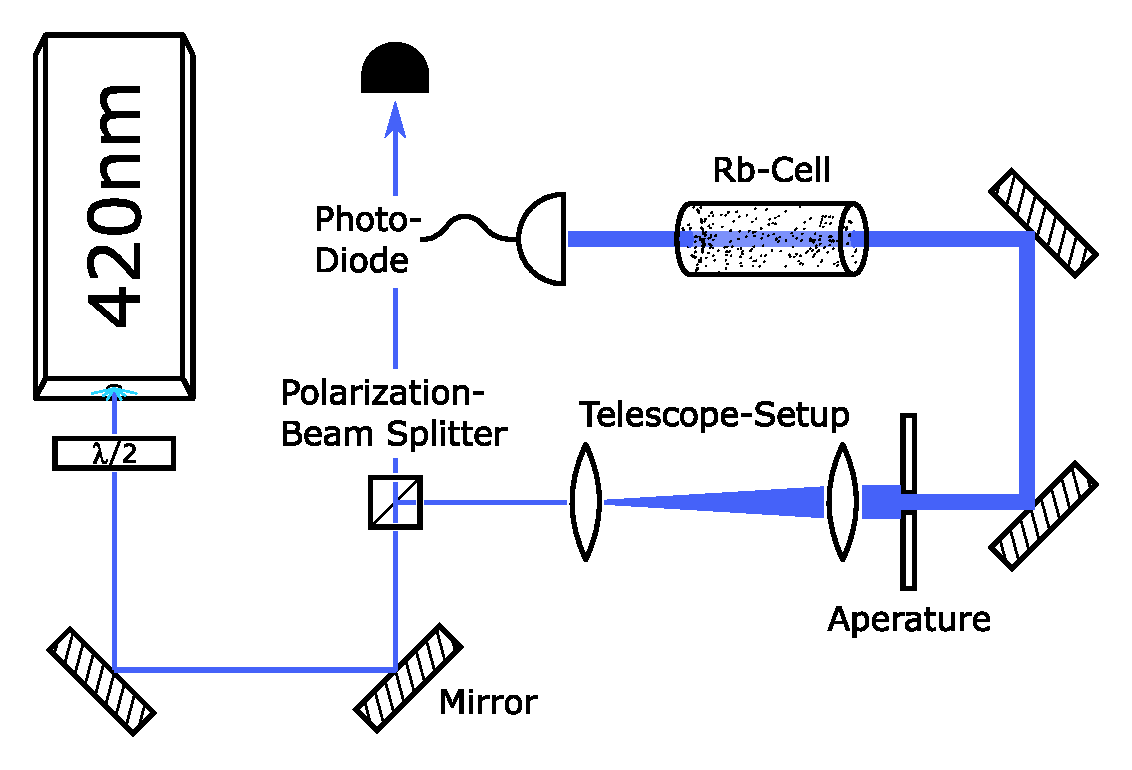
\includegraphics[width=0.6\textwidth]{absorption_spectroscopy}    
    \caption{\label{fig:absorption_spectroscopy_setup} Setup for an absorption 
    spectroscopy.}
\end{figure}

\begin{wrapfigure}{Hr}{.4\textwidth}
    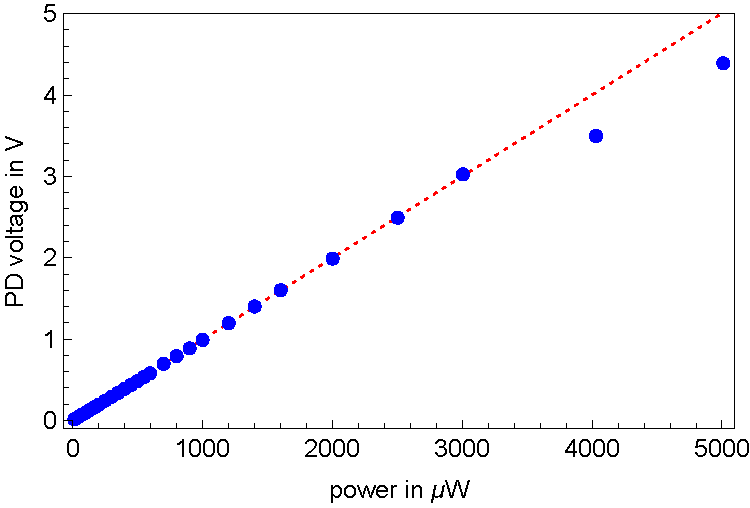
\includegraphics[width=0.35\textwidth]{pd_check}    
    \caption{\label{fig:pd_check} Maximum PD voltage taken out of atomic resonance 
    over power measured before the cell to ensure PD linearity; measurements at 
    \SI{4000}{\micro\watt} and \SI{5000}{\micro\watt} will be excluded.}
    \vspace{2em}
    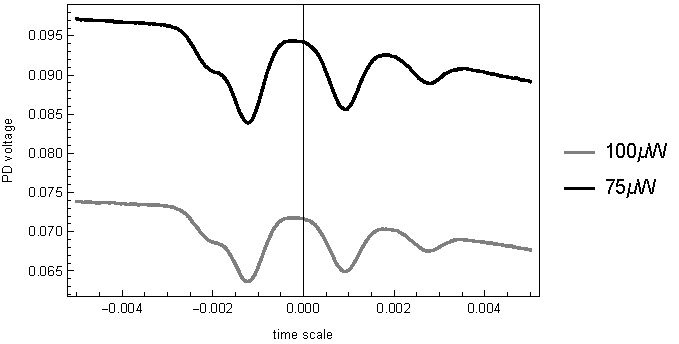
\includegraphics[width=0.35\textwidth]{power_compare}    
    \caption{\label{fig:power_compare} Absorption spectra at \SI{75}{\micro\watt}
    and \SI{100}{\micro\watt}.}
\end{wrapfigure}
We want to measure the intensity after the cell as a function of the initial
intensity \(I_0\). The transmitted intensity depends on the detuning as shown in
formula~\ref{eq:kappa_final}. \\
We will thus scan the laser frequency across the atomic resonances and for each 
input power record the signal using a photodiode (PD) 
(see Fig.~\ref{fig:absorption_spectroscopy_setup}) connected to a Teledyne Lecroy 
HDO6000A a digital storage oscilloscope. The PD records a signal 
proportional to the intensity only for a given range of power, so we made sure 
that we where using the PD in the linear range (see Fig.~\ref{fig:pd_check}). The
gain of the PD was adjusted in order to not saturate the signal, but to have the
widest possible dynamics to obtain the best signal to noise ratio. To 
change the input power, we turned the \(\lambda/2\) plate before the polarizing 
beam splitter (PBS) and measured it before every spectroscopy. It should be noted 
that changes of the sensor position in between measurements and variation of the
remaining ambient light lead to an increasing uncertainty at lower beam power. 
We account for \SI{10}{\percent} uncertainty below \SI{100}{\micro\watt}, 
\SI{8}{\percent} below \SI{250}{\micro\watt}, \SI{6}{\percent} below 
\SI{1000}{\micro\watt} and \SI{3}{\percent} above.\\
Before the spectroscopy itself, after the power was measured, the heating system,
due to its noise generating magnetic field, and all lights besides the measuring 
equipment were turned off. The spectroscopy was performed by scanning the laser 
wavelength using the piezo scanning option of the DL pro controller. We centered 
the scan range for all the measurements using the controller and the oscilloscope. 
For each input power we recorded the spectra and saved it onto a USB stick for 
further data analysis. We followed a logarithmic progression for the power 
increments from \SIrange{13}{5000}{\micro\watt}. Two examples of the recorded 
spectrum are shown in Fig.~\ref{fig:power_compare}. The choice of the power 
together with the beam cross section, should enable to probe intensity range from 
below to above \(I_{s}\). \\
In the next chapter we will discuss the analysis of the gathered data. 




%!TEX root = ../thesis.tex
% Spellcheck ignore
% cSpell:ignore freerunning, detuning, microresonator, misestimates, Mathematica, modelfit, kappaplot, isat, powermeter, mathrm, giga, kappamodelratio, realrubidium, hyperfine, kappacorrection, intcorrection, powercorrection, multicolumn, extracolsep, toprule, midrule, bottomrule, fitplot, gaussians, nonumber, spectrumlegend, FWHM, diaminplot, meanplot, diaplot, bigskip, captionof, minipage, pagebreak, wincam, includegraphics,wrapfigure, ifpdf, graphicspath
%*******************************************************************************
%****************************** Fourth Chapter *********************************
%*******************************************************************************
\chapter{Evaluation}

% **************************** Define Graphics Path **************************
\ifpdf{}
    \graphicspath{{Chapter4/Figs/Raster/}{Chapter4/Figs/PDF/}{Chapter4/Figs/}}
\else
    \graphicspath{{Chapter4/Figs/Vector/}{Chapter4/Figs/}}
\fi

The scanning span we used was more than the \SI{6.86}{\giga\hertz} of the hyperfine
splitting of \(^{87}\)Rb. We thus observe four absorption dips due to \(^{87}\)Rb 
\(F=1\) and \(F=2\) and \(^{85}\)Rb \(F=2\) and \(F=3\). In the data analysis,
we treated each of the dips as a two-level atom, using the theory described in
Chapter 2.\\
We are interested in determining \(I_{s}\), which is included in \(\kappa'_0 \)
(see Eq.~\ref{eq:kappa_final}). We will use the Beer-Lambert law 
\( I(x)=I_0~\mathrm{e}^{-\kappa x} \), which leads on resonance to
\begin{align}
    I(x,\nu_0) = I_0~\mathrm{e}^{-\kappa'_0 x}~.
\end{align}
Which gives us an expression for \(\kappa'_0\)
\begin{align}\label{eq:kappa_prime}
    \kappa'_0 = -\frac{1}{L}~\ln\left(\frac{I(L,\nu_0)}{I_0} \right)
\end{align}
where \(L\) is the cell length. \\
Thus, one needs to extract from the absorption spectroscopy dips \(I(L,\nu_0) \)
and \(I_0\). We measured \(I(L,\nu_0,I_0) \) for different values of \(I_0\) and 
computed the experimental \(\kappa_0\). We will then fit the theory formula
~\ref{eq:kappa_final} using \(I_{s}\) and \(T\) as free parameters to extract 
them for the four ``atoms''. 

\pagebreak
%********************************** % First Section  **************************************
\section{Model fit on absorption spectra}~\label{sec:modelfit} %Section - 4.1
\begin{figure}[H]
    \centering
    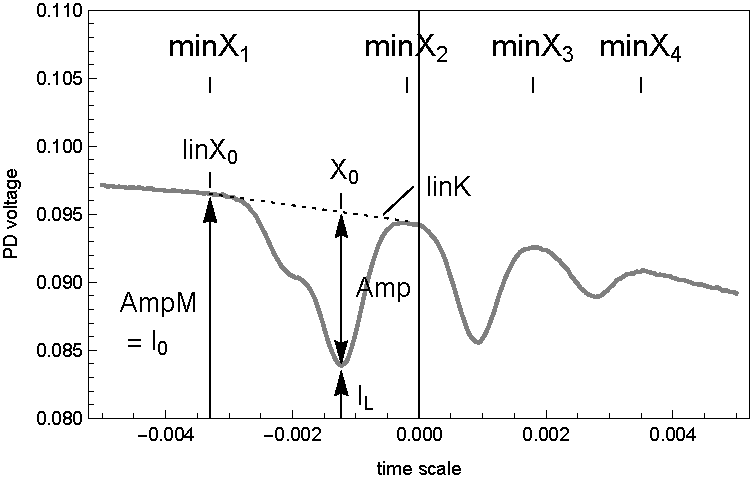
\includegraphics[width=.6\textwidth]{spectrumlegend}
    \caption{\label{fig:spectrumlegend} Definition of all model parameters for the
    \(^{85}\)Rb \(F=3\) line.}
\end{figure}

The whole data analysis and parameter fitting has been made using mathematica.
To narrow down the range for our fits of the different lines we defined four
constants \(minX_1\) to \(minX_4\) which mark the beginning or the end of one dip. 
As can be seen in Equation~\ref{eq:kappa_final} all our spectra are based on a 
gaussian model, but due to the short separation of the \(^{87}\)Rb \(F=2\) and 
\(^{85}\)Rb \(F=3\) line we have also an overlapping double gaussian. To reduce 
mode hopping the laser adjusted the beam power during the scan and therefore our 
spectra have a linear decrease in power. Our fitting models are based on a double 
and two single gaussians. For the explanation of all the parameters we will use 
the \(^{85}\)Rb \(F=3\) line as an example (see Fig.~\ref{fig:spectrumlegend}).
\begin{align}
    Gauss1 &= AmpM-Amp\cdot Exp\left(-\frac{{(x-x_0)}^2}{2~\sigma^2} \right) +
                linK(x-linX_0)  \\
    Gauss2 &= AmpM-Amp1\cdot Exp\left(-\frac{{(x-x_1)}^2}{2~{\sigma_1}^2} \right)-
                  Amp2\cdot Exp\left(-\frac{{(x-x_2)}^2}{2~{\sigma_2}^2} \right) \nonumber \\
                  &+ linK(x-linX_0)~,
\end{align}
where \(AmpM\) is the maximum power without absorption, \(Amp\) is the amplitude 
of the absorption, \(x_0\) is the center of the absorption line, \(\sigma \) is 
the standard deviation of the gaussian, \(linK\) is the slope of the power 
decrease and \(linX_0\) is the beginning of the gaussian. In case of the double 
gaussian the different parameters of the gaussians are labeled with the indices 
``1'' and ``2''.\\
With these two models all the spectra where fitted and the obtained parameters 
where saved into a single table for further analysis. The error bars of the
fits where saved into a separate table, which we will use for the uncertainties
of the absorption coefficient. One example of the fitted models is shown 
in Fig.~\ref{fig:fitplot}. All the info we want is contained in \(AmpM\) and \(Amp\).
\begin{figure}[H]
    \centering
    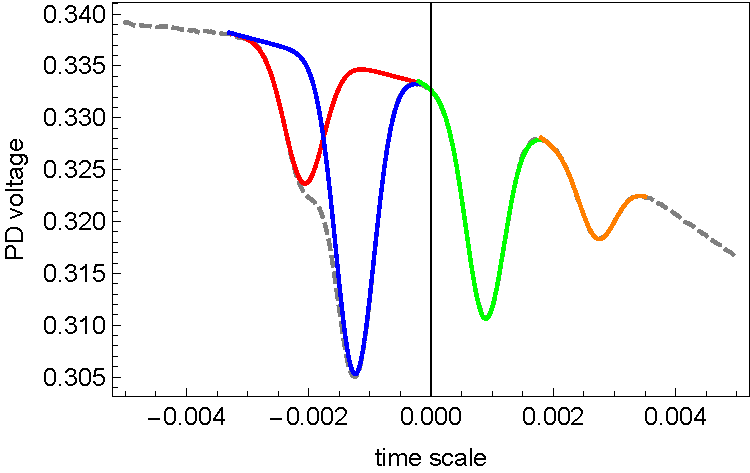
\includegraphics[width=.8\textwidth]{fitplot}
    \caption{\label{fig:fitplot} Absorption spectrum at \SI{350}{\micro\watt}
    with the fitted absorption lines.}
\end{figure}

\pagebreak
%********************************** % Second Section  **************************************
\section{Power extraction} %Section - 4.2

To link \(AmpM\) to the power measured with the powermeter, we need to take into
account that the power measured before the cell corresponds to the mean value
over the scanning range. For that reason we calculated the power at each transition 
position, assuming a linear decline and considering that the mean value lies in 
the middle of the minimum and maximum power (see Fig.~\ref{fig:powercorrection}). 
We applied these corrections for all our data sets. An example of the extracted 
powers can be found in Table.~\ref{table:powercorrection}. The error bars come 
from the powermeter uncertainties.

\begin{figure}[H]
    \centering
    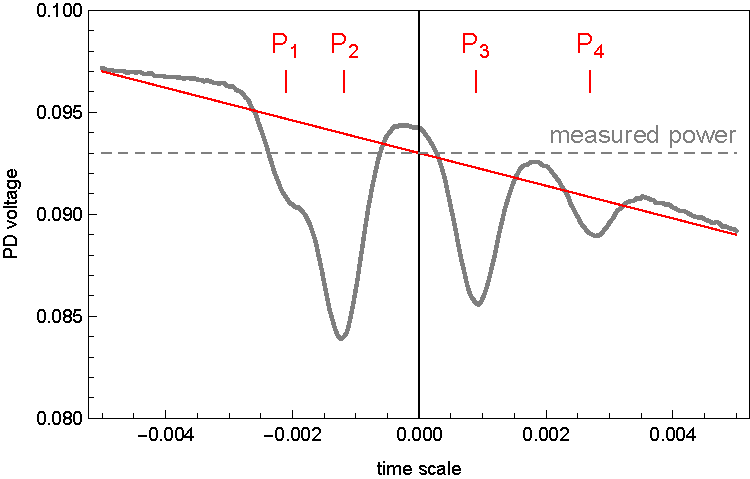
\includegraphics[width=.7\textwidth]{powercorrection}
    \caption{\label{fig:powercorrection} Linear approximation on power decrease}
\end{figure}

\begin{table}[h]
    \centering
    \begin{tabular*}{0.7\textwidth}{@{\extracolsep{\fill} }l c c}
    \toprule
    measured power: \SI{350}{\micro\watt} & & \\
    \midrule
    line & power [\si{\micro\watt}] & uncertainty [\si{\micro\watt}] \\
    \midrule
    \(^{87}\)Rb \(F=2\) & 355 & 21 \\
    \(^{85}\)Rb \(F=3\) & 353 & 21 \\
    \(^{85}\)Rb \(F=2\) & 347 & 20 \\
    \(^{87}\)Rb \(F=1\) & 343 & 20 \\
    \bottomrule
    \end{tabular*}
    \caption{\label{table:powercorrection} Power correction for \SI{350}{\micro\watt}
    measurement.}
\end{table}
\pagebreak
%********************************** % Third Section  **************************************
\section{Measured absorption coefficient} %Section - 4.3

To determine the absorption coefficient, we have to calculate the 
intensity for all transitions and measurements. For this we will use the 
estimated cross section of Section~\ref{sec:laser_dia_measurement} and the flat 
hat model \(I = \frac{power}{cross~section}\). The error bars are based on the
uncertainties of the power measurement given in Section~\ref{sec:absorption_spec}.
As an example the calculated intensities for the \SI{350}{\micro\watt} measurement 
can be found in Table~\ref{table:intcorrection}.

\bigskip
\begin{table}[h]
    \centering
    \begin{tabular*}{0.7\textwidth}{@{\extracolsep{\fill} }l c c}
    \toprule
    \multicolumn{3}{l}{calculated intensity at \SI{350}{\micro\watt}: \SI{168}{\watt\per\meter\squared}} \\
    \midrule
    line & intensity [\si{\watt\per\meter\squared}] & uncertainty [\si{\watt\per\meter\squared}] \\
    \midrule
    \(^{87}\)Rb \(F=2\) & 170 & 14 \\
    \(^{85}\)Rb \(F=3\) & 169 & 14 \\
    \(^{85}\)Rb \(F=2\) & 167 & 14 \\
    \(^{87}\)Rb \(F=1\) & 165 & 14 \\
    \bottomrule
    \end{tabular*}
    \caption{\label{table:intcorrection} Corresponding intensities to the power
    correction of the \SI{350}{\micro\watt} measurement.}
\end{table}

With Equation~\ref{eq:kappa_prime} and the length of the rubidium cell (\(L=\SI{0.1}{\meter}\))
one can now determine \(\kappa'_0\) for all lines and measurements.
As we can see in Fig.~\ref{fig:spectrumlegend} \(I_0\) corresponds to \(AmpM\)
and \(I(L,\nu_0)\) to \(AmpM-Amp\). It should be noted that we make an error on the 
assumption of \(AmpM~\widehat{=}~I_0 \), because of the linear decrease of 
amplitude/power over \(\nu \) (see Fig.~\ref{fig:powercorrection}).
We can limit the maximum error to \SI{3}{\percent}, due to the fact that the 
maximum relative amplitude deviation over the whole spectrum is on average \SI{6}{\percent}. 
This will be taken into account for the calculation of \(\kappa \). The uncertainties
for the different absorption coefficients are based on the uncertainties of the 
gaussian fit of the spectrum, which where extracted in Section~\ref{sec:modelfit}.
An example for the measured absorption coefficient is given in 
Table.~\ref{table:kappacorrection}.

\bigskip
\begin{table}[h]
    \centering
    \begin{tabular*}{0.7\textwidth}{@{\extracolsep{\fill} }l c c}
    \toprule
    \multicolumn{3}{l}{absorption coefficients at \SI{350}{\micro\watt} } \\
    \midrule
    line & \(\kappa \) [\si{\per\meter}] & uncertainty [\si{\per\meter}] \\
    \midrule
    \(^{87}\)Rb \(F=2\) & 0.38 & \num{0.17e-3} \\
    \(^{85}\)Rb \(F=3\) & 0.92 & \num{0.19e-3} \\
    \(^{85}\)Rb \(F=2\) & 0.62 & \num{0.20e-3} \\
    \(^{87}\)Rb \(F=1\) & 0.21 & \num{0.13e-3} \\
    \bottomrule
    \end{tabular*}
    \caption{\label{table:kappacorrection} Calculated absorption coefficients
    for \SI{350}{\micro\watt} measurement.}
\end{table}

The absorption coefficients calculated from our spectroscopy will then be fitted 
to the theoretical ones. 

%********************************** % Forth Section  **************************************
\section{Saturation intensity determination} %Section - 4.4

To account for isotope proportions and hyperfine level populations 
(see Sec.~\ref{sec:realrubidium}), each of the absorption coefficient models for 
our fit will be balanced, because it changes the atom density \(n_0\). In detail, we have a vapor constituted 
of the two atoms in two states each and their abundance depend on isotope 
concentration and on atom \(m_F\) level population. So we have
\begin{align}
    n_{0,tot} = n_{0,^{87}Rb~F=2} + n_{0,^{85}Rb~F=3} + n_{0,^{85}Rb~F=2} +
    n_{0,^{87}Rb~F=1}~.
\end{align} 
Where for each atom \(n_0\) is replaced by \(n_{0,tot} \times ratio_X \) 
(see Table.~\ref{table:kappamodelratio})

\bigskip
\begin{table}[h]
    \centering
    \begin{tabular*}{0.8\textwidth}{@{\extracolsep{\fill} }l c c c}
    \toprule
    \multicolumn{4}{l}{\(\kappa \) model adaptation} \\
    \midrule
    line & isotope abundance & hyperfine levels & \(ratio_X\) \\
    \midrule
    \(^{87}\)Rb \(F=2\) & 0.2784 & 5/8 & 0.174 \\
    \(^{85}\)Rb \(F=3\) & 0.7216 & 7/12 & 0.421\\
    \(^{85}\)Rb \(F=2\) & 0.7216 & 5/12 & 0.301\\
    \(^{87}\)Rb \(F=1\) & 0.2784 & 3/8 & 0.104 \\
    \midrule
    & & & 1.000 \\
    \bottomrule
    \end{tabular*}
    \caption{\label{table:kappamodelratio} Atomic density ratios of the different
    isotopes and hyperfine lines}
\end{table}

This leads to our model based on Equation~\ref{eq:kappa_final}

\begin{align}
    \kappa'_{0,X} = n_{0,tot} ~ratio_X ~ \frac{\pi^2 {\Gamma_\nu}^2}{I_{s}}~ h~\nu_0 ~ 
    \frac{c}{\nu_0} ~ \sqrt{ \frac{m_X}{2\pi~k_B T} } ~
    \frac{1}{\sqrt{1 + \frac{2I}{I_s}~\frac{\Gamma_\nu}{\Gamma_{\nu,tot}}}}~, 
\end{align}

where \(X\) stands for the different lines. The total atom density \(n_{0,tot} \) 
can be extracted out of the vapor-pressure model~\cite{vapour_pres}:
\begin{align}
    \log_{10} P_V = 4.312-\frac{4040}{T}~,
\end{align}
where \(P_V \) is the pressure in atmospheres and the ideal gas law, such that
\begin{align}
    n_{0,tot} = \frac{1}{k_B T}~10^{9.318-\frac{4040}{T}}~.
\end{align}

We use Mathematica to fit our data and because we want to include the obtained
error bars for the fit, we are restricted to a NonlinearModelFit. Moreover it is
only possible to have error bars on the y-axis of your data, which will be 
incorporated via a weight on every data point. For this reason we had to choose
the measurement with the larger error bars as our y-axis. We can see in our 
calculation that the error bars on \(\kappa \) are two orders of magnitude smaller 
than the errors bars on the calculated intensity 
(see Tables~\ref{table:intcorrection} and~\ref{table:kappacorrection}). However 
our models are \(\kappa \) depending on \(I \). For that reason we have to exchange
x- and y-axis of the used data sets and invert our model so we get \(I(\kappa)\) 
instead of \(\kappa(I)\).\\
To extract \(\kappa \) of our measurements we used the Beer-Lambert law, which 
assumes that \(\kappa \) is independent from \(I\). This assumption is only true
for intensities below \(I_{s}\). Therefore we have to limit our measurement data 
where the initial intensity is below \(I_{s} = \SI{126}{\watt\per\meter\squared}\), 
which is the theoretical one (see Fig.~\ref{fig:kappaplot}). Therefore we get 
following values and corresponding error bars for \(I_{s}\) and temperature 
\(T\) for every absorption line extracted (see Table~\ref{table:isat_temp}):

\bigskip
\begin{table}[h]
    \centering
    \begin{tabular*}{0.9\textwidth}{@{\extracolsep{\fill} }l c c c c}
    \toprule
    \multicolumn{5}{l}{saturation intensity and temperature} \\
    \midrule
    line & \(I_{s}\) [\si{\watt\per\meter\squared}] & uncertainty [\si{\watt\per\meter\squared}] &
           \(T \) [\si{\kelvin}] & uncertainty [\si{\kelvin}] \\
    \midrule
    \(^{87}\)Rb \(F=2\) & 45.6 & 1.8 & 336.9 & 0.4 \\
    \(^{85}\)Rb \(F=3\) & 51.7 & 2.5 & 338.2 & 0.5 \\
    \(^{85}\)Rb \(F=2\) & 37.2 & 2.6 & 334.5 & 0.6 \\
    \(^{87}\)Rb \(F=1\) & 30.7 & 3.3 & 332.3 & 0.9 \\
    \midrule
    mean value  & 41.3 & & 335.5 & \\
    \bottomrule
    \end{tabular*}
    \caption{\label{table:isat_temp} Fitted values of \(I_{s}\) and temperature.}
\end{table}

\begin{figure}[H]
    \centering
    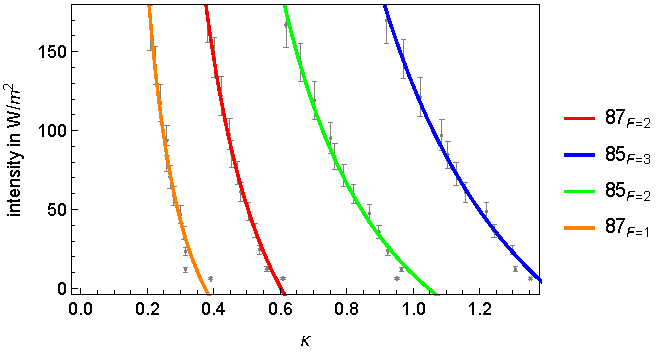
\includegraphics[width=.8\textwidth]{kappaplot}
    \caption{\label{fig:kappaplot} Plot of the four inverted absorption coefficients
    with corresponding error bars}
\end{figure}


%\include{Chapter5/chapter5}
%\include{Chapter6/chapter6}
%\include{Chapter7/chapter7}



% ********************************** Back Matter *******************************
% Backmatter should be commented out, if you are using appendices after References
%\backmatter

% ********************************** Bibliography ******************************
\begin{spacing}{0.9}

% To use the conventional natbib style referencing
% Bibliography style previews: http://nodonn.tipido.net/bibstyle.php
% Reference styles: http://sites.stat.psu.edu/~surajit/present/bib.htm

\bibliographystyle{unsrt}
%\bibliographystyle{unsrt} % Use for unsorted references  
%\bibliographystyle{plainnat} % use this to have URLs listed in References
\cleardoublepage{}
\bibliography{References/references} % Path to your References.bib file


% If you would like to use BibLaTeX for your references, pass `custombib' as
% an option in the document class. The location of 'reference.bib' should be
% specified in the preamble.tex file in the custombib section.
% Comment out the lines related to natbib above and uncomment the following line.

%\printbibliography[heading=bibintoc, title={References}]


\end{spacing}

% ********************************** Appendices ********************************

\begin{appendices} % Using appendices environment for more functionality

%!TEX root = ../thesis.tex
% ******************************* Thesis Appendix A ****************************
\chapter{Theory} 


%!TEX root = ../thesis.tex
% ******************************* Thesis Appendix B ********************************

\chapter{Experiment}


%!TEX root = ../thesis.tex
% ******************************* Thesis Appendix C ****************************
\chapter{Evaluation} 



\end{appendices}

% *************************************** Index ********************************
\printthesisindex{} % If index is present

\end{document}
